% Created by tikzDevice version 0.12.5 on 2023-10-26 18:48:00
% !TEX encoding = UTF-8 Unicode
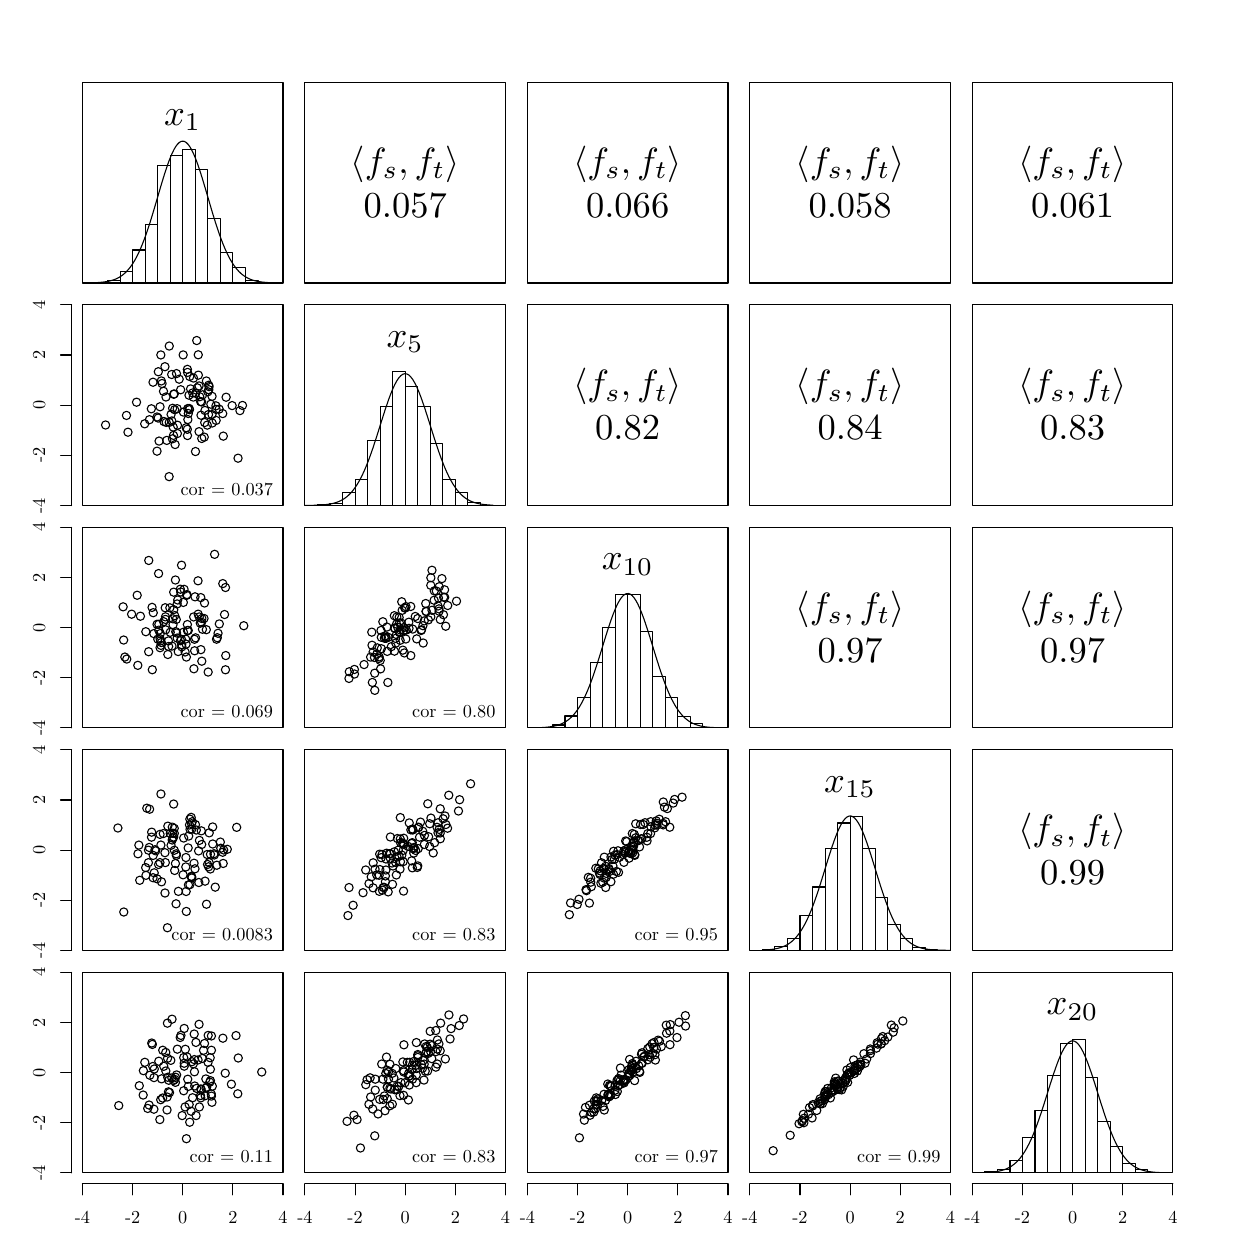
\begin{tikzpicture}[x=1pt,y=1pt]
\definecolor{fillColor}{RGB}{255,255,255}
\path[use as bounding box,fill=fillColor,fill opacity=0.00] (0,0) rectangle (433.62,433.62);
\begin{scope}
\path[clip] (  0.00,  0.00) rectangle (433.62,433.62);
\definecolor{drawColor}{RGB}{0,0,0}

\path[draw=drawColor,line width= 0.4pt,line join=round,line cap=round] ( 19.80,341.35) --
	( 92.27,341.35) --
	( 92.27,413.82) --
	( 19.80,413.82) --
	cycle;
\end{scope}
\begin{scope}
\path[clip] ( 19.80,341.35) rectangle ( 92.27,413.82);
\definecolor{drawColor}{RGB}{0,0,0}

\path[draw=drawColor,line width= 0.4pt,line join=round,line cap=round] ( 24.33,341.35) rectangle ( 28.86,341.61);

\path[draw=drawColor,line width= 0.4pt,line join=round,line cap=round] ( 28.86,341.35) rectangle ( 33.39,342.29);

\path[draw=drawColor,line width= 0.4pt,line join=round,line cap=round] ( 33.39,341.35) rectangle ( 37.92,345.38);

\path[draw=drawColor,line width= 0.4pt,line join=round,line cap=round] ( 37.92,341.35) rectangle ( 42.45,353.26);

\path[draw=drawColor,line width= 0.4pt,line join=round,line cap=round] ( 42.45,341.35) rectangle ( 46.98,362.60);

\path[draw=drawColor,line width= 0.4pt,line join=round,line cap=round] ( 46.98,341.35) rectangle ( 51.50,383.67);

\path[draw=drawColor,line width= 0.4pt,line join=round,line cap=round] ( 51.50,341.35) rectangle ( 56.03,387.44);

\path[draw=drawColor,line width= 0.4pt,line join=round,line cap=round] ( 56.03,341.35) rectangle ( 60.56,389.66);

\path[draw=drawColor,line width= 0.4pt,line join=round,line cap=round] ( 60.56,341.35) rectangle ( 65.09,382.21);

\path[draw=drawColor,line width= 0.4pt,line join=round,line cap=round] ( 65.09,341.35) rectangle ( 69.62,364.65);

\path[draw=drawColor,line width= 0.4pt,line join=round,line cap=round] ( 69.62,341.35) rectangle ( 74.15,352.32);

\path[draw=drawColor,line width= 0.4pt,line join=round,line cap=round] ( 74.15,341.35) rectangle ( 78.68,347.09);

\path[draw=drawColor,line width= 0.4pt,line join=round,line cap=round] ( 78.68,341.35) rectangle ( 83.21,342.12);

\path[draw=drawColor,line width= 0.4pt,line join=round,line cap=round] ( 83.21,341.35) rectangle ( 87.74,341.61);

\path[draw=drawColor,line width= 0.4pt,line join=round,line cap=round] ( 24.33,341.46) --
	( 24.96,341.49) --
	( 25.60,341.53) --
	( 26.23,341.58) --
	( 26.87,341.64) --
	( 27.50,341.71) --
	( 28.13,341.80) --
	( 28.77,341.90) --
	( 29.40,342.03) --
	( 30.04,342.19) --
	( 30.67,342.37) --
	( 31.30,342.59) --
	( 31.94,342.84) --
	( 32.57,343.14) --
	( 33.21,343.49) --
	( 33.84,343.90) --
	( 34.47,344.37) --
	( 35.11,344.91) --
	( 35.74,345.52) --
	( 36.38,346.22) --
	( 37.01,347.00) --
	( 37.65,347.88) --
	( 38.28,348.86) --
	( 38.91,349.94) --
	( 39.55,351.14) --
	( 40.18,352.44) --
	( 40.82,353.85) --
	( 41.45,355.38) --
	( 42.08,357.01) --
	( 42.72,358.75) --
	( 43.35,360.59) --
	( 43.99,362.52) --
	( 44.62,364.53) --
	( 45.25,366.60) --
	( 45.89,368.73) --
	( 46.52,370.89) --
	( 47.16,373.06) --
	( 47.79,375.23) --
	( 48.42,377.37) --
	( 49.06,379.46) --
	( 49.69,381.47) --
	( 50.33,383.39) --
	( 50.96,385.17) --
	( 51.60,386.81) --
	( 52.23,388.28) --
	( 52.86,389.57) --
	( 53.50,390.64) --
	( 54.13,391.49) --
	( 54.77,392.11) --
	( 55.40,392.49) --
	( 56.03,392.61) --
	( 56.67,392.49) --
	( 57.30,392.11) --
	( 57.94,391.49) --
	( 58.57,390.64) --
	( 59.20,389.57) --
	( 59.84,388.28) --
	( 60.47,386.81) --
	( 61.11,385.17) --
	( 61.74,383.39) --
	( 62.37,381.47) --
	( 63.01,379.46) --
	( 63.64,377.37) --
	( 64.28,375.23) --
	( 64.91,373.06) --
	( 65.55,370.89) --
	( 66.18,368.73) --
	( 66.81,366.60) --
	( 67.45,364.53) --
	( 68.08,362.52) --
	( 68.72,360.59) --
	( 69.35,358.75) --
	( 69.98,357.01) --
	( 70.62,355.38) --
	( 71.25,353.85) --
	( 71.89,352.44) --
	( 72.52,351.14) --
	( 73.15,349.94) --
	( 73.79,348.86) --
	( 74.42,347.88) --
	( 75.06,347.00) --
	( 75.69,346.22) --
	( 76.33,345.52) --
	( 76.96,344.91) --
	( 77.59,344.37) --
	( 78.23,343.90) --
	( 78.86,343.49) --
	( 79.50,343.14) --
	( 80.13,342.84) --
	( 80.76,342.59) --
	( 81.40,342.37) --
	( 82.03,342.19) --
	( 82.67,342.03) --
	( 83.30,341.90) --
	( 83.93,341.80) --
	( 84.57,341.71) --
	( 85.20,341.64) --
	( 85.84,341.58) --
	( 86.47,341.53) --
	( 87.10,341.49) --
	( 87.74,341.46);
\end{scope}
\begin{scope}
\path[clip] (  0.00,  0.00) rectangle (433.62,433.62);
\definecolor{drawColor}{RGB}{0,0,0}

\path[draw=drawColor,line width= 0.4pt,line join=round,line cap=round] ( 19.80, 15.84) -- ( 92.27, 15.84);

\path[draw=drawColor,line width= 0.4pt,line join=round,line cap=round] ( 19.80, 15.84) -- ( 19.80, 11.88);

\path[draw=drawColor,line width= 0.4pt,line join=round,line cap=round] ( 37.92, 15.84) -- ( 37.92, 11.88);

\path[draw=drawColor,line width= 0.4pt,line join=round,line cap=round] ( 56.03, 15.84) -- ( 56.03, 11.88);

\path[draw=drawColor,line width= 0.4pt,line join=round,line cap=round] ( 74.15, 15.84) -- ( 74.15, 11.88);

\path[draw=drawColor,line width= 0.4pt,line join=round,line cap=round] ( 92.27, 15.84) -- ( 92.27, 11.88);

\node[text=drawColor,anchor=base,inner sep=0pt, outer sep=0pt, scale=  0.66] at ( 19.80,  1.58) {-4};

\node[text=drawColor,anchor=base,inner sep=0pt, outer sep=0pt, scale=  0.66] at ( 37.92,  1.58) {-2};

\node[text=drawColor,anchor=base,inner sep=0pt, outer sep=0pt, scale=  0.66] at ( 56.03,  1.58) {0};

\node[text=drawColor,anchor=base,inner sep=0pt, outer sep=0pt, scale=  0.66] at ( 74.15,  1.58) {2};

\node[text=drawColor,anchor=base,inner sep=0pt, outer sep=0pt, scale=  0.66] at ( 92.27,  1.58) {4};
\end{scope}
\begin{scope}
\path[clip] ( 19.80,341.35) rectangle ( 92.27,413.82);
\definecolor{drawColor}{RGB}{0,0,0}

\node[text=drawColor,anchor=base,inner sep=0pt, outer sep=0pt, scale=  1.32] at ( 56.03,398.44) {$x_{1}$};
\end{scope}
\begin{scope}
\path[clip] (  0.00,  0.00) rectangle (433.62,433.62);
\definecolor{drawColor}{RGB}{0,0,0}

\path[draw=drawColor,line width= 0.4pt,line join=round,line cap=round] ( 19.80,260.96) --
	( 92.27,260.96) --
	( 92.27,333.43) --
	( 19.80,333.43) --
	cycle;
\end{scope}
\begin{scope}
\path[clip] ( 19.80,260.96) rectangle ( 92.27,333.43);
\definecolor{drawColor}{RGB}{0,0,0}

\path[draw=drawColor,line width= 0.4pt,line join=round,line cap=round] ( 58.47,295.58) circle (  1.49);

\path[draw=drawColor,line width= 0.4pt,line join=round,line cap=round] ( 58.87,303.09) circle (  1.49);

\path[draw=drawColor,line width= 0.4pt,line join=round,line cap=round] ( 42.28,290.47) circle (  1.49);

\path[draw=drawColor,line width= 0.4pt,line join=round,line cap=round] ( 55.28,302.78) circle (  1.49);

\path[draw=drawColor,line width= 0.4pt,line join=round,line cap=round] ( 62.90,285.18) circle (  1.49);

\path[draw=drawColor,line width= 0.4pt,line join=round,line cap=round] ( 45.30,305.50) circle (  1.49);

\path[draw=drawColor,line width= 0.4pt,line join=round,line cap=round] ( 58.56,307.58) circle (  1.49);

\path[draw=drawColor,line width= 0.4pt,line join=round,line cap=round] ( 35.70,293.50) circle (  1.49);

\path[draw=drawColor,line width= 0.4pt,line join=round,line cap=round] ( 54.13,289.96) circle (  1.49);

\path[draw=drawColor,line width= 0.4pt,line join=round,line cap=round] ( 57.71,310.15) circle (  1.49);

\path[draw=drawColor,line width= 0.4pt,line join=round,line cap=round] ( 73.88,297.05) circle (  1.49);

\path[draw=drawColor,line width= 0.4pt,line join=round,line cap=round] ( 69.20,295.78) circle (  1.49);

\path[draw=drawColor,line width= 0.4pt,line join=round,line cap=round] ( 57.84,295.97) circle (  1.49);

\path[draw=drawColor,line width= 0.4pt,line join=round,line cap=round] ( 44.69,295.90) circle (  1.49);

\path[draw=drawColor,line width= 0.4pt,line join=round,line cap=round] ( 64.06,295.30) circle (  1.49);

\path[draw=drawColor,line width= 0.4pt,line join=round,line cap=round] ( 56.26,294.72) circle (  1.49);

\path[draw=drawColor,line width= 0.4pt,line join=round,line cap=round] ( 61.93,287.64) circle (  1.49);

\path[draw=drawColor,line width= 0.4pt,line join=round,line cap=round] ( 76.70,295.24) circle (  1.49);

\path[draw=drawColor,line width= 0.4pt,line join=round,line cap=round] ( 28.15,290.04) circle (  1.49);

\path[draw=drawColor,line width= 0.4pt,line join=round,line cap=round] ( 48.56,305.03) circle (  1.49);

\path[draw=drawColor,line width= 0.4pt,line join=round,line cap=round] ( 70.48,294.17) circle (  1.49);

\path[draw=drawColor,line width= 0.4pt,line join=round,line cap=round] ( 47.83,296.64) circle (  1.49);

\path[draw=drawColor,line width= 0.4pt,line join=round,line cap=round] ( 52.59,289.28) circle (  1.49);

\path[draw=drawColor,line width= 0.4pt,line join=round,line cap=round] ( 65.35,293.82) circle (  1.49);

\path[draw=drawColor,line width= 0.4pt,line join=round,line cap=round] ( 52.03,308.29) circle (  1.49);

\path[draw=drawColor,line width= 0.4pt,line join=round,line cap=round] ( 53.12,295.57) circle (  1.49);

\path[draw=drawColor,line width= 0.4pt,line join=round,line cap=round] ( 62.64,293.58) circle (  1.49);

\path[draw=drawColor,line width= 0.4pt,line join=round,line cap=round] ( 58.29,300.81) circle (  1.49);

\path[draw=drawColor,line width= 0.4pt,line join=round,line cap=round] ( 68.09,295.68) circle (  1.49);

\path[draw=drawColor,line width= 0.4pt,line join=round,line cap=round] ( 36.24,287.44) circle (  1.49);

\path[draw=drawColor,line width= 0.4pt,line join=round,line cap=round] ( 61.09,320.56) circle (  1.49);

\path[draw=drawColor,line width= 0.4pt,line join=round,line cap=round] ( 65.42,304.42) circle (  1.49);

\path[draw=drawColor,line width= 0.4pt,line join=round,line cap=round] ( 48.29,305.97) circle (  1.49);

\path[draw=drawColor,line width= 0.4pt,line join=round,line cap=round] ( 70.69,286.02) circle (  1.49);

\path[draw=drawColor,line width= 0.4pt,line join=round,line cap=round] ( 47.15,292.55) circle (  1.49);

\path[draw=drawColor,line width= 0.4pt,line join=round,line cap=round] ( 64.89,290.00) circle (  1.49);

\path[draw=drawColor,line width= 0.4pt,line join=round,line cap=round] ( 53.28,282.99) circle (  1.49);

\path[draw=drawColor,line width= 0.4pt,line join=round,line cap=round] ( 52.32,285.04) circle (  1.49);

\path[draw=drawColor,line width= 0.4pt,line join=round,line cap=round] ( 77.62,297.11) circle (  1.49);

\path[draw=drawColor,line width= 0.4pt,line join=round,line cap=round] ( 47.21,309.29) circle (  1.49);

\path[draw=drawColor,line width= 0.4pt,line join=round,line cap=round] ( 68.03,296.96) circle (  1.49);

\path[draw=drawColor,line width= 0.4pt,line join=round,line cap=round] ( 51.16,318.57) circle (  1.49);

\path[draw=drawColor,line width= 0.4pt,line join=round,line cap=round] ( 39.34,298.28) circle (  1.49);

\path[draw=drawColor,line width= 0.4pt,line join=round,line cap=round] ( 52.69,286.30) circle (  1.49);

\path[draw=drawColor,line width= 0.4pt,line join=round,line cap=round] ( 52.97,301.27) circle (  1.49);

\path[draw=drawColor,line width= 0.4pt,line join=round,line cap=round] ( 76.02,278.05) circle (  1.49);

\path[draw=drawColor,line width= 0.4pt,line join=round,line cap=round] ( 46.75,292.94) circle (  1.49);

\path[draw=drawColor,line width= 0.4pt,line join=round,line cap=round] ( 57.75,286.23) circle (  1.49);

\path[draw=drawColor,line width= 0.4pt,line join=round,line cap=round] ( 60.64,280.45) circle (  1.49);

\path[draw=drawColor,line width= 0.4pt,line join=round,line cap=round] ( 64.58,305.95) circle (  1.49);

\path[draw=drawColor,line width= 0.4pt,line join=round,line cap=round] ( 54.75,306.60) circle (  1.49);

\path[draw=drawColor,line width= 0.4pt,line join=round,line cap=round] ( 71.71,300.08) circle (  1.49);

\path[draw=drawColor,line width= 0.4pt,line join=round,line cap=round] ( 54.09,286.96) circle (  1.49);

\path[draw=drawColor,line width= 0.4pt,line join=round,line cap=round] ( 46.74,280.59) circle (  1.49);

\path[draw=drawColor,line width= 0.4pt,line join=round,line cap=round] ( 62.17,300.26) circle (  1.49);

\path[draw=drawColor,line width= 0.4pt,line join=round,line cap=round] ( 57.28,289.06) circle (  1.49);

\path[draw=drawColor,line width= 0.4pt,line join=round,line cap=round] ( 65.46,302.79) circle (  1.49);

\path[draw=drawColor,line width= 0.4pt,line join=round,line cap=round] ( 62.86,298.36) circle (  1.49);

\path[draw=drawColor,line width= 0.4pt,line join=round,line cap=round] ( 61.68,308.06) circle (  1.49);

\path[draw=drawColor,line width= 0.4pt,line join=round,line cap=round] ( 66.19,297.57) circle (  1.49);

\path[draw=drawColor,line width= 0.4pt,line join=round,line cap=round] ( 52.10,291.51) circle (  1.49);

\path[draw=drawColor,line width= 0.4pt,line join=round,line cap=round] ( 63.21,300.94) circle (  1.49);

\path[draw=drawColor,line width= 0.4pt,line join=round,line cap=round] ( 59.92,307.00) circle (  1.49);

\path[draw=drawColor,line width= 0.4pt,line join=round,line cap=round] ( 57.76,309.05) circle (  1.49);

\path[draw=drawColor,line width= 0.4pt,line join=round,line cap=round] ( 63.97,290.94) circle (  1.49);

\path[draw=drawColor,line width= 0.4pt,line join=round,line cap=round] ( 57.88,292.01) circle (  1.49);

\path[draw=drawColor,line width= 0.4pt,line join=round,line cap=round] ( 51.11,271.39) circle (  1.49);

\path[draw=drawColor,line width= 0.4pt,line join=round,line cap=round] ( 50.05,290.98) circle (  1.49);

\path[draw=drawColor,line width= 0.4pt,line join=round,line cap=round] ( 61.64,315.41) circle (  1.49);

\path[draw=drawColor,line width= 0.4pt,line join=round,line cap=round] ( 47.48,284.23) circle (  1.49);

\path[draw=drawColor,line width= 0.4pt,line join=round,line cap=round] ( 66.68,290.76) circle (  1.49);

\path[draw=drawColor,line width= 0.4pt,line join=round,line cap=round] ( 49.23,291.30) circle (  1.49);

\path[draw=drawColor,line width= 0.4pt,line join=round,line cap=round] ( 65.56,303.90) circle (  1.49);

\path[draw=drawColor,line width= 0.4pt,line join=round,line cap=round] ( 62.49,298.51) circle (  1.49);

\path[draw=drawColor,line width= 0.4pt,line join=round,line cap=round] ( 54.02,295.94) circle (  1.49);

\path[draw=drawColor,line width= 0.4pt,line join=round,line cap=round] ( 59.85,300.12) circle (  1.49);

\path[draw=drawColor,line width= 0.4pt,line join=round,line cap=round] ( 51.83,293.88) circle (  1.49);

\path[draw=drawColor,line width= 0.4pt,line join=round,line cap=round] ( 58.05,294.20) circle (  1.49);

\path[draw=drawColor,line width= 0.4pt,line join=round,line cap=round] ( 61.31,303.46) circle (  1.49);

\path[draw=drawColor,line width= 0.4pt,line join=round,line cap=round] ( 53.77,308.61) circle (  1.49);

\path[draw=drawColor,line width= 0.4pt,line join=round,line cap=round] ( 57.70,288.49) circle (  1.49);

\path[draw=drawColor,line width= 0.4pt,line join=round,line cap=round] ( 63.80,285.66) circle (  1.49);

\path[draw=drawColor,line width= 0.4pt,line join=round,line cap=round] ( 52.38,296.09) circle (  1.49);

\path[draw=drawColor,line width= 0.4pt,line join=round,line cap=round] ( 49.60,311.11) circle (  1.49);

\path[draw=drawColor,line width= 0.4pt,line join=round,line cap=round] ( 66.60,293.83) circle (  1.49);

\path[draw=drawColor,line width= 0.4pt,line join=round,line cap=round] ( 68.10,291.70) circle (  1.49);

\path[draw=drawColor,line width= 0.4pt,line join=round,line cap=round] ( 52.75,301.16) circle (  1.49);

\path[draw=drawColor,line width= 0.4pt,line join=round,line cap=round] ( 49.97,300.16) circle (  1.49);

\path[draw=drawColor,line width= 0.4pt,line join=round,line cap=round] ( 60.71,301.48) circle (  1.49);

\path[draw=drawColor,line width= 0.4pt,line join=round,line cap=round] ( 56.18,315.37) circle (  1.49);

\path[draw=drawColor,line width= 0.4pt,line join=round,line cap=round] ( 61.93,304.16) circle (  1.49);

\path[draw=drawColor,line width= 0.4pt,line join=round,line cap=round] ( 51.16,290.99) circle (  1.49);

\path[draw=drawColor,line width= 0.4pt,line join=round,line cap=round] ( 65.11,302.06) circle (  1.49);

\path[draw=drawColor,line width= 0.4pt,line join=round,line cap=round] ( 44.00,291.96) circle (  1.49);

\path[draw=drawColor,line width= 0.4pt,line join=round,line cap=round] ( 49.08,302.22) circle (  1.49);

\path[draw=drawColor,line width= 0.4pt,line join=round,line cap=round] ( 66.63,300.40) circle (  1.49);

\path[draw=drawColor,line width= 0.4pt,line join=round,line cap=round] ( 58.35,296.01) circle (  1.49);

\path[draw=drawColor,line width= 0.4pt,line join=round,line cap=round] ( 48.12,315.36) circle (  1.49);

\path[draw=drawColor,line width= 0.4pt,line join=round,line cap=round] ( 59.62,301.62) circle (  1.49);

\path[draw=drawColor,line width= 0.4pt,line join=round,line cap=round] ( 50.27,284.48) circle (  1.49);

\node[text=drawColor,anchor=base east,inner sep=0pt, outer sep=0pt, scale=  0.66] at ( 88.64,264.59) {cor = 0.037};
\end{scope}
\begin{scope}
\path[clip] (  0.00,  0.00) rectangle (433.62,433.62);
\definecolor{drawColor}{RGB}{0,0,0}

\path[draw=drawColor,line width= 0.4pt,line join=round,line cap=round] ( 15.84,260.96) -- ( 15.84,333.43);

\path[draw=drawColor,line width= 0.4pt,line join=round,line cap=round] ( 15.84,260.96) -- ( 11.88,260.96);

\path[draw=drawColor,line width= 0.4pt,line join=round,line cap=round] ( 15.84,279.08) -- ( 11.88,279.08);

\path[draw=drawColor,line width= 0.4pt,line join=round,line cap=round] ( 15.84,297.20) -- ( 11.88,297.20);

\path[draw=drawColor,line width= 0.4pt,line join=round,line cap=round] ( 15.84,315.32) -- ( 11.88,315.32);

\path[draw=drawColor,line width= 0.4pt,line join=round,line cap=round] ( 15.84,333.43) -- ( 11.88,333.43);

\node[text=drawColor,rotate= 90.00,anchor=base,inner sep=0pt, outer sep=0pt, scale=  0.66] at (  6.34,260.96) {-4};

\node[text=drawColor,rotate= 90.00,anchor=base,inner sep=0pt, outer sep=0pt, scale=  0.66] at (  6.34,279.08) {-2};

\node[text=drawColor,rotate= 90.00,anchor=base,inner sep=0pt, outer sep=0pt, scale=  0.66] at (  6.34,297.20) {0};

\node[text=drawColor,rotate= 90.00,anchor=base,inner sep=0pt, outer sep=0pt, scale=  0.66] at (  6.34,315.32) {2};

\node[text=drawColor,rotate= 90.00,anchor=base,inner sep=0pt, outer sep=0pt, scale=  0.66] at (  6.34,333.43) {4};
\end{scope}
\begin{scope}
\path[clip] (  0.00,  0.00) rectangle (433.62,433.62);
\definecolor{drawColor}{RGB}{0,0,0}

\path[draw=drawColor,line width= 0.4pt,line join=round,line cap=round] ( 19.80,180.58) --
	( 92.27,180.58) --
	( 92.27,253.04) --
	( 19.80,253.04) --
	cycle;
\end{scope}
\begin{scope}
\path[clip] ( 19.80,180.58) rectangle ( 92.27,253.04);
\definecolor{drawColor}{RGB}{0,0,0}

\path[draw=drawColor,line width= 0.4pt,line join=round,line cap=round] ( 53.39,234.03) circle (  1.49);

\path[draw=drawColor,line width= 0.4pt,line join=round,line cap=round] ( 55.55,212.62) circle (  1.49);

\path[draw=drawColor,line width= 0.4pt,line join=round,line cap=round] ( 49.70,224.00) circle (  1.49);

\path[draw=drawColor,line width= 0.4pt,line join=round,line cap=round] ( 48.30,211.43) circle (  1.49);

\path[draw=drawColor,line width= 0.4pt,line join=round,line cap=round] ( 57.43,228.49) circle (  1.49);

\path[draw=drawColor,line width= 0.4pt,line join=round,line cap=round] ( 59.97,220.70) circle (  1.49);

\path[draw=drawColor,line width= 0.4pt,line join=round,line cap=round] ( 51.51,215.13) circle (  1.49);

\path[draw=drawColor,line width= 0.4pt,line join=round,line cap=round] ( 51.38,223.98) circle (  1.49);

\path[draw=drawColor,line width= 0.4pt,line join=round,line cap=round] ( 56.89,208.03) circle (  1.49);

\path[draw=drawColor,line width= 0.4pt,line join=round,line cap=round] ( 47.99,212.02) circle (  1.49);

\path[draw=drawColor,line width= 0.4pt,line join=round,line cap=round] ( 55.21,212.10) circle (  1.49);

\path[draw=drawColor,line width= 0.4pt,line join=round,line cap=round] ( 39.57,228.52) circle (  1.49);

\path[draw=drawColor,line width= 0.4pt,line join=round,line cap=round] ( 47.40,218.02) circle (  1.49);

\path[draw=drawColor,line width= 0.4pt,line join=round,line cap=round] ( 53.69,219.78) circle (  1.49);

\path[draw=drawColor,line width= 0.4pt,line join=round,line cap=round] ( 53.13,221.16) circle (  1.49);

\path[draw=drawColor,line width= 0.4pt,line join=round,line cap=round] ( 78.09,217.51) circle (  1.49);

\path[draw=drawColor,line width= 0.4pt,line join=round,line cap=round] ( 45.60,214.67) circle (  1.49);

\path[draw=drawColor,line width= 0.4pt,line join=round,line cap=round] ( 65.21,200.77) circle (  1.49);

\path[draw=drawColor,line width= 0.4pt,line join=round,line cap=round] ( 62.37,218.44) circle (  1.49);

\path[draw=drawColor,line width= 0.4pt,line join=round,line cap=round] ( 57.71,217.93) circle (  1.49);

\path[draw=drawColor,line width= 0.4pt,line join=round,line cap=round] ( 35.80,205.46) circle (  1.49);

\path[draw=drawColor,line width= 0.4pt,line join=round,line cap=round] ( 52.46,220.00) circle (  1.49);

\path[draw=drawColor,line width= 0.4pt,line join=round,line cap=round] ( 53.81,214.90) circle (  1.49);

\path[draw=drawColor,line width= 0.4pt,line join=round,line cap=round] ( 57.35,206.19) circle (  1.49);

\path[draw=drawColor,line width= 0.4pt,line join=round,line cap=round] ( 60.33,208.46) circle (  1.49);

\path[draw=drawColor,line width= 0.4pt,line join=round,line cap=round] ( 42.70,215.35) circle (  1.49);

\path[draw=drawColor,line width= 0.4pt,line join=round,line cap=round] ( 45.38,222.22) circle (  1.49);

\path[draw=drawColor,line width= 0.4pt,line join=round,line cap=round] ( 39.80,203.19) circle (  1.49);

\path[draw=drawColor,line width= 0.4pt,line join=round,line cap=round] ( 71.48,201.59) circle (  1.49);

\path[draw=drawColor,line width= 0.4pt,line join=round,line cap=round] ( 50.65,207.12) circle (  1.49);

\path[draw=drawColor,line width= 0.4pt,line join=round,line cap=round] ( 57.72,215.78) circle (  1.49);

\path[draw=drawColor,line width= 0.4pt,line join=round,line cap=round] ( 44.95,224.14) circle (  1.49);

\path[draw=drawColor,line width= 0.4pt,line join=round,line cap=round] ( 52.52,217.91) circle (  1.49);

\path[draw=drawColor,line width= 0.4pt,line join=round,line cap=round] ( 52.15,210.15) circle (  1.49);

\path[draw=drawColor,line width= 0.4pt,line join=round,line cap=round] ( 60.06,201.95) circle (  1.49);

\path[draw=drawColor,line width= 0.4pt,line join=round,line cap=round] ( 68.79,214.77) circle (  1.49);

\path[draw=drawColor,line width= 0.4pt,line join=round,line cap=round] ( 49.76,219.80) circle (  1.49);

\path[draw=drawColor,line width= 0.4pt,line join=round,line cap=round] ( 43.75,241.10) circle (  1.49);

\path[draw=drawColor,line width= 0.4pt,line join=round,line cap=round] ( 63.16,216.24) circle (  1.49);

\path[draw=drawColor,line width= 0.4pt,line join=round,line cap=round] ( 56.52,230.66) circle (  1.49);

\path[draw=drawColor,line width= 0.4pt,line join=round,line cap=round] ( 57.23,210.86) circle (  1.49);

\path[draw=drawColor,line width= 0.4pt,line join=round,line cap=round] ( 53.51,215.37) circle (  1.49);

\path[draw=drawColor,line width= 0.4pt,line join=round,line cap=round] ( 69.25,218.17) circle (  1.49);

\path[draw=drawColor,line width= 0.4pt,line join=round,line cap=round] ( 34.49,224.34) circle (  1.49);

\path[draw=drawColor,line width= 0.4pt,line join=round,line cap=round] ( 68.25,212.64) circle (  1.49);

\path[draw=drawColor,line width= 0.4pt,line join=round,line cap=round] ( 50.94,210.03) circle (  1.49);

\path[draw=drawColor,line width= 0.4pt,line join=round,line cap=round] ( 62.94,220.12) circle (  1.49);

\path[draw=drawColor,line width= 0.4pt,line join=round,line cap=round] ( 56.28,215.16) circle (  1.49);

\path[draw=drawColor,line width= 0.4pt,line join=round,line cap=round] ( 62.92,204.70) circle (  1.49);

\path[draw=drawColor,line width= 0.4pt,line join=round,line cap=round] ( 61.56,233.74) circle (  1.49);

\path[draw=drawColor,line width= 0.4pt,line join=round,line cap=round] ( 45.04,201.61) circle (  1.49);

\path[draw=drawColor,line width= 0.4pt,line join=round,line cap=round] ( 50.87,212.03) circle (  1.49);

\path[draw=drawColor,line width= 0.4pt,line join=round,line cap=round] ( 63.72,220.14) circle (  1.49);

\path[draw=drawColor,line width= 0.4pt,line join=round,line cap=round] ( 34.68,212.34) circle (  1.49);

\path[draw=drawColor,line width= 0.4pt,line join=round,line cap=round] ( 57.07,212.70) circle (  1.49);

\path[draw=drawColor,line width= 0.4pt,line join=round,line cap=round] ( 67.55,243.31) circle (  1.49);

\path[draw=drawColor,line width= 0.4pt,line join=round,line cap=round] ( 62.59,208.87) circle (  1.49);

\path[draw=drawColor,line width= 0.4pt,line join=round,line cap=round] ( 57.56,228.77) circle (  1.49);

\path[draw=drawColor,line width= 0.4pt,line join=round,line cap=round] ( 54.39,208.18) circle (  1.49);

\path[draw=drawColor,line width= 0.4pt,line join=round,line cap=round] ( 71.48,231.32) circle (  1.49);

\path[draw=drawColor,line width= 0.4pt,line join=round,line cap=round] ( 55.63,210.65) circle (  1.49);

\path[draw=drawColor,line width= 0.4pt,line join=round,line cap=round] ( 55.60,239.38) circle (  1.49);

\path[draw=drawColor,line width= 0.4pt,line join=round,line cap=round] ( 54.22,226.81) circle (  1.49);

\path[draw=drawColor,line width= 0.4pt,line join=round,line cap=round] ( 71.58,206.73) circle (  1.49);

\path[draw=drawColor,line width= 0.4pt,line join=round,line cap=round] ( 63.90,225.72) circle (  1.49);

\path[draw=drawColor,line width= 0.4pt,line join=round,line cap=round] ( 54.02,213.05) circle (  1.49);

\path[draw=drawColor,line width= 0.4pt,line join=round,line cap=round] ( 49.85,216.03) circle (  1.49);

\path[draw=drawColor,line width= 0.4pt,line join=round,line cap=round] ( 60.47,227.95) circle (  1.49);

\path[draw=drawColor,line width= 0.4pt,line join=round,line cap=round] ( 47.86,212.80) circle (  1.49);

\path[draw=drawColor,line width= 0.4pt,line join=round,line cap=round] ( 62.56,227.67) circle (  1.49);

\path[draw=drawColor,line width= 0.4pt,line join=round,line cap=round] ( 55.72,209.88) circle (  1.49);

\path[draw=drawColor,line width= 0.4pt,line join=round,line cap=round] ( 47.31,236.35) circle (  1.49);

\path[draw=drawColor,line width= 0.4pt,line join=round,line cap=round] ( 62.85,218.75) circle (  1.49);

\path[draw=drawColor,line width= 0.4pt,line join=round,line cap=round] ( 70.50,232.73) circle (  1.49);

\path[draw=drawColor,line width= 0.4pt,line join=round,line cap=round] ( 60.68,213.13) circle (  1.49);

\path[draw=drawColor,line width= 0.4pt,line join=round,line cap=round] ( 56.25,225.94) circle (  1.49);

\path[draw=drawColor,line width= 0.4pt,line join=round,line cap=round] ( 37.56,221.68) circle (  1.49);

\path[draw=drawColor,line width= 0.4pt,line join=round,line cap=round] ( 62.01,220.69) circle (  1.49);

\path[draw=drawColor,line width= 0.4pt,line join=round,line cap=round] ( 47.91,214.68) circle (  1.49);

\path[draw=drawColor,line width= 0.4pt,line join=round,line cap=round] ( 52.76,229.64) circle (  1.49);

\path[draw=drawColor,line width= 0.4pt,line join=round,line cap=round] ( 47.37,215.91) circle (  1.49);

\path[draw=drawColor,line width= 0.4pt,line join=round,line cap=round] ( 68.52,213.18) circle (  1.49);

\path[draw=drawColor,line width= 0.4pt,line join=round,line cap=round] ( 64.55,216.08) circle (  1.49);

\path[draw=drawColor,line width= 0.4pt,line join=round,line cap=round] ( 58.02,215.79) circle (  1.49);

\path[draw=drawColor,line width= 0.4pt,line join=round,line cap=round] ( 46.76,218.02) circle (  1.49);

\path[draw=drawColor,line width= 0.4pt,line join=round,line cap=round] ( 60.27,212.62) circle (  1.49);

\path[draw=drawColor,line width= 0.4pt,line join=round,line cap=round] ( 61.61,221.69) circle (  1.49);

\path[draw=drawColor,line width= 0.4pt,line join=round,line cap=round] ( 55.31,229.70) circle (  1.49);

\path[draw=drawColor,line width= 0.4pt,line join=round,line cap=round] ( 71.14,221.56) circle (  1.49);

\path[draw=drawColor,line width= 0.4pt,line join=round,line cap=round] ( 48.16,210.42) circle (  1.49);

\path[draw=drawColor,line width= 0.4pt,line join=round,line cap=round] ( 55.17,230.71) circle (  1.49);

\path[draw=drawColor,line width= 0.4pt,line join=round,line cap=round] ( 52.78,223.32) circle (  1.49);

\path[draw=drawColor,line width= 0.4pt,line join=round,line cap=round] ( 47.02,212.66) circle (  1.49);

\path[draw=drawColor,line width= 0.4pt,line join=round,line cap=round] ( 35.12,206.19) circle (  1.49);

\path[draw=drawColor,line width= 0.4pt,line join=round,line cap=round] ( 43.72,208.12) circle (  1.49);

\path[draw=drawColor,line width= 0.4pt,line join=round,line cap=round] ( 47.84,209.57) circle (  1.49);

\path[draw=drawColor,line width= 0.4pt,line join=round,line cap=round] ( 49.79,220.72) circle (  1.49);

\path[draw=drawColor,line width= 0.4pt,line join=round,line cap=round] ( 49.13,218.97) circle (  1.49);

\path[draw=drawColor,line width= 0.4pt,line join=round,line cap=round] ( 40.74,220.95) circle (  1.49);

\path[draw=drawColor,line width= 0.4pt,line join=round,line cap=round] ( 54.01,225.38) circle (  1.49);

\node[text=drawColor,anchor=base east,inner sep=0pt, outer sep=0pt, scale=  0.66] at ( 88.64,184.20) {cor = 0.069};
\end{scope}
\begin{scope}
\path[clip] (  0.00,  0.00) rectangle (433.62,433.62);
\definecolor{drawColor}{RGB}{0,0,0}

\path[draw=drawColor,line width= 0.4pt,line join=round,line cap=round] ( 15.84,180.58) -- ( 15.84,253.04);

\path[draw=drawColor,line width= 0.4pt,line join=round,line cap=round] ( 15.84,180.58) -- ( 11.88,180.58);

\path[draw=drawColor,line width= 0.4pt,line join=round,line cap=round] ( 15.84,198.69) -- ( 11.88,198.69);

\path[draw=drawColor,line width= 0.4pt,line join=round,line cap=round] ( 15.84,216.81) -- ( 11.88,216.81);

\path[draw=drawColor,line width= 0.4pt,line join=round,line cap=round] ( 15.84,234.93) -- ( 11.88,234.93);

\path[draw=drawColor,line width= 0.4pt,line join=round,line cap=round] ( 15.84,253.04) -- ( 11.88,253.04);

\node[text=drawColor,rotate= 90.00,anchor=base,inner sep=0pt, outer sep=0pt, scale=  0.66] at (  6.34,180.58) {-4};

\node[text=drawColor,rotate= 90.00,anchor=base,inner sep=0pt, outer sep=0pt, scale=  0.66] at (  6.34,198.69) {-2};

\node[text=drawColor,rotate= 90.00,anchor=base,inner sep=0pt, outer sep=0pt, scale=  0.66] at (  6.34,216.81) {0};

\node[text=drawColor,rotate= 90.00,anchor=base,inner sep=0pt, outer sep=0pt, scale=  0.66] at (  6.34,234.93) {2};

\node[text=drawColor,rotate= 90.00,anchor=base,inner sep=0pt, outer sep=0pt, scale=  0.66] at (  6.34,253.04) {4};
\end{scope}
\begin{scope}
\path[clip] (  0.00,  0.00) rectangle (433.62,433.62);
\definecolor{drawColor}{RGB}{0,0,0}

\path[draw=drawColor,line width= 0.4pt,line join=round,line cap=round] ( 19.80,100.19) --
	( 92.27,100.19) --
	( 92.27,172.66) --
	( 19.80,172.66) --
	cycle;
\end{scope}
\begin{scope}
\path[clip] ( 19.80,100.19) rectangle ( 92.27,172.66);
\definecolor{drawColor}{RGB}{0,0,0}

\path[draw=drawColor,line width= 0.4pt,line join=round,line cap=round] ( 52.99,136.37) circle (  1.49);

\path[draw=drawColor,line width= 0.4pt,line join=round,line cap=round] ( 60.94,143.68) circle (  1.49);

\path[draw=drawColor,line width= 0.4pt,line join=round,line cap=round] ( 49.60,135.50) circle (  1.49);

\path[draw=drawColor,line width= 0.4pt,line join=round,line cap=round] ( 44.80,142.92) circle (  1.49);

\path[draw=drawColor,line width= 0.4pt,line join=round,line cap=round] ( 53.62,117.02) circle (  1.49);

\path[draw=drawColor,line width= 0.4pt,line join=round,line cap=round] ( 49.62,120.93) circle (  1.49);

\path[draw=drawColor,line width= 0.4pt,line join=round,line cap=round] ( 58.60,147.63) circle (  1.49);

\path[draw=drawColor,line width= 0.4pt,line join=round,line cap=round] ( 60.63,145.65) circle (  1.49);

\path[draw=drawColor,line width= 0.4pt,line join=round,line cap=round] ( 59.30,144.01) circle (  1.49);

\path[draw=drawColor,line width= 0.4pt,line join=round,line cap=round] ( 32.60,144.42) circle (  1.49);

\path[draw=drawColor,line width= 0.4pt,line join=round,line cap=round] ( 50.65,145.09) circle (  1.49);

\path[draw=drawColor,line width= 0.4pt,line join=round,line cap=round] ( 52.26,144.73) circle (  1.49);

\path[draw=drawColor,line width= 0.4pt,line join=round,line cap=round] ( 67.78,123.05) circle (  1.49);

\path[draw=drawColor,line width= 0.4pt,line join=round,line cap=round] ( 66.85,144.80) circle (  1.49);

\path[draw=drawColor,line width= 0.4pt,line join=round,line cap=round] ( 40.18,138.24) circle (  1.49);

\path[draw=drawColor,line width= 0.4pt,line join=round,line cap=round] ( 64.10,125.22) circle (  1.49);

\path[draw=drawColor,line width= 0.4pt,line join=round,line cap=round] ( 75.52,144.66) circle (  1.49);

\path[draw=drawColor,line width= 0.4pt,line join=round,line cap=round] ( 42.75,127.32) circle (  1.49);

\path[draw=drawColor,line width= 0.4pt,line join=round,line cap=round] ( 52.22,140.08) circle (  1.49);

\path[draw=drawColor,line width= 0.4pt,line join=round,line cap=round] ( 43.05,151.58) circle (  1.49);

\path[draw=drawColor,line width= 0.4pt,line join=round,line cap=round] ( 57.14,130.35) circle (  1.49);

\path[draw=drawColor,line width= 0.4pt,line join=round,line cap=round] ( 59.08,148.26) circle (  1.49);

\path[draw=drawColor,line width= 0.4pt,line join=round,line cap=round] ( 58.47,145.53) circle (  1.49);

\path[draw=drawColor,line width= 0.4pt,line join=round,line cap=round] ( 62.05,139.94) circle (  1.49);

\path[draw=drawColor,line width= 0.4pt,line join=round,line cap=round] ( 65.57,131.92) circle (  1.49);

\path[draw=drawColor,line width= 0.4pt,line join=round,line cap=round] ( 62.88,138.46) circle (  1.49);

\path[draw=drawColor,line width= 0.4pt,line join=round,line cap=round] ( 46.72,126.08) circle (  1.49);

\path[draw=drawColor,line width= 0.4pt,line join=round,line cap=round] ( 62.74,143.39) circle (  1.49);

\path[draw=drawColor,line width= 0.4pt,line join=round,line cap=round] ( 59.47,146.68) circle (  1.49);

\path[draw=drawColor,line width= 0.4pt,line join=round,line cap=round] ( 65.60,142.67) circle (  1.49);

\path[draw=drawColor,line width= 0.4pt,line join=round,line cap=round] ( 48.14,138.26) circle (  1.49);

\path[draw=drawColor,line width= 0.4pt,line join=round,line cap=round] ( 53.12,129.08) circle (  1.49);

\path[draw=drawColor,line width= 0.4pt,line join=round,line cap=round] ( 52.40,142.54) circle (  1.49);

\path[draw=drawColor,line width= 0.4pt,line join=round,line cap=round] ( 45.35,134.51) circle (  1.49);

\path[draw=drawColor,line width= 0.4pt,line join=round,line cap=round] ( 70.65,131.61) circle (  1.49);

\path[draw=drawColor,line width= 0.4pt,line join=round,line cap=round] ( 59.24,126.76) circle (  1.49);

\path[draw=drawColor,line width= 0.4pt,line join=round,line cap=round] ( 49.75,131.92) circle (  1.49);

\path[draw=drawColor,line width= 0.4pt,line join=round,line cap=round] ( 56.37,140.80) circle (  1.49);

\path[draw=drawColor,line width= 0.4pt,line join=round,line cap=round] ( 66.06,134.93) circle (  1.49);

\path[draw=drawColor,line width= 0.4pt,line join=round,line cap=round] ( 50.50,108.38) circle (  1.49);

\path[draw=drawColor,line width= 0.4pt,line join=round,line cap=round] ( 65.37,130.40) circle (  1.49);

\path[draw=drawColor,line width= 0.4pt,line join=round,line cap=round] ( 69.77,137.10) circle (  1.49);

\path[draw=drawColor,line width= 0.4pt,line join=round,line cap=round] ( 48.36,124.97) circle (  1.49);

\path[draw=drawColor,line width= 0.4pt,line join=round,line cap=round] ( 52.96,144.30) circle (  1.49);

\path[draw=drawColor,line width= 0.4pt,line join=round,line cap=round] ( 53.68,135.09) circle (  1.49);

\path[draw=drawColor,line width= 0.4pt,line join=round,line cap=round] ( 48.15,156.71) circle (  1.49);

\path[draw=drawColor,line width= 0.4pt,line join=round,line cap=round] ( 58.09,123.85) circle (  1.49);

\path[draw=drawColor,line width= 0.4pt,line join=round,line cap=round] ( 68.34,130.97) circle (  1.49);

\path[draw=drawColor,line width= 0.4pt,line join=round,line cap=round] ( 59.23,145.97) circle (  1.49);

\path[draw=drawColor,line width= 0.4pt,line join=round,line cap=round] ( 57.19,133.75) circle (  1.49);

\path[draw=drawColor,line width= 0.4pt,line join=round,line cap=round] ( 52.75,141.15) circle (  1.49);

\path[draw=drawColor,line width= 0.4pt,line join=round,line cap=round] ( 56.16,127.51) circle (  1.49);

\path[draw=drawColor,line width= 0.4pt,line join=round,line cap=round] ( 61.85,124.72) circle (  1.49);

\path[draw=drawColor,line width= 0.4pt,line join=round,line cap=round] ( 57.26,121.48) circle (  1.49);

\path[draw=drawColor,line width= 0.4pt,line join=round,line cap=round] ( 49.00,142.40) circle (  1.49);

\path[draw=drawColor,line width= 0.4pt,line join=round,line cap=round] ( 57.32,114.27) circle (  1.49);

\path[draw=drawColor,line width= 0.4pt,line join=round,line cap=round] ( 47.83,142.12) circle (  1.49);

\path[draw=drawColor,line width= 0.4pt,line join=round,line cap=round] ( 58.68,143.94) circle (  1.49);

\path[draw=drawColor,line width= 0.4pt,line join=round,line cap=round] ( 43.64,136.41) circle (  1.49);

\path[draw=drawColor,line width= 0.4pt,line join=round,line cap=round] ( 34.73,114.06) circle (  1.49);

\path[draw=drawColor,line width= 0.4pt,line join=round,line cap=round] ( 58.18,141.51) circle (  1.49);

\path[draw=drawColor,line width= 0.4pt,line join=round,line cap=round] ( 66.01,129.61) circle (  1.49);

\path[draw=drawColor,line width= 0.4pt,line join=round,line cap=round] ( 53.39,131.58) circle (  1.49);

\path[draw=drawColor,line width= 0.4pt,line join=round,line cap=round] ( 53.73,134.52) circle (  1.49);

\path[draw=drawColor,line width= 0.4pt,line join=round,line cap=round] ( 51.52,142.45) circle (  1.49);

\path[draw=drawColor,line width= 0.4pt,line join=round,line cap=round] ( 39.85,135.10) circle (  1.49);

\path[draw=drawColor,line width= 0.4pt,line join=round,line cap=round] ( 52.75,153.07) circle (  1.49);

\path[draw=drawColor,line width= 0.4pt,line join=round,line cap=round] ( 70.83,136.47) circle (  1.49);

\path[draw=drawColor,line width= 0.4pt,line join=round,line cap=round] ( 40.49,125.52) circle (  1.49);

\path[draw=drawColor,line width= 0.4pt,line join=round,line cap=round] ( 61.76,136.14) circle (  1.49);

\path[draw=drawColor,line width= 0.4pt,line join=round,line cap=round] ( 46.01,136.56) circle (  1.49);

\path[draw=drawColor,line width= 0.4pt,line join=round,line cap=round] ( 64.87,134.84) circle (  1.49);

\path[draw=drawColor,line width= 0.4pt,line join=round,line cap=round] ( 52.99,142.46) circle (  1.49);

\path[draw=drawColor,line width= 0.4pt,line join=round,line cap=round] ( 47.79,131.91) circle (  1.49);

\path[draw=drawColor,line width= 0.4pt,line join=round,line cap=round] ( 59.29,126.35) circle (  1.49);

\path[draw=drawColor,line width= 0.4pt,line join=round,line cap=round] ( 72.13,136.72) circle (  1.49);

\path[draw=drawColor,line width= 0.4pt,line join=round,line cap=round] ( 57.99,137.22) circle (  1.49);

\path[draw=drawColor,line width= 0.4pt,line join=round,line cap=round] ( 70.45,135.66) circle (  1.49);

\path[draw=drawColor,line width= 0.4pt,line join=round,line cap=round] ( 69.62,139.33) circle (  1.49);

\path[draw=drawColor,line width= 0.4pt,line join=round,line cap=round] ( 66.87,138.64) circle (  1.49);

\path[draw=drawColor,line width= 0.4pt,line join=round,line cap=round] ( 54.46,121.52) circle (  1.49);

\path[draw=drawColor,line width= 0.4pt,line join=round,line cap=round] ( 60.12,131.69) circle (  1.49);

\path[draw=drawColor,line width= 0.4pt,line join=round,line cap=round] ( 42.64,130.11) circle (  1.49);

\path[draw=drawColor,line width= 0.4pt,line join=round,line cap=round] ( 67.33,135.13) circle (  1.49);

\path[draw=drawColor,line width= 0.4pt,line join=round,line cap=round] ( 64.62,116.88) circle (  1.49);

\path[draw=drawColor,line width= 0.4pt,line join=round,line cap=round] ( 43.62,131.88) circle (  1.49);

\path[draw=drawColor,line width= 0.4pt,line join=round,line cap=round] ( 51.82,138.17) circle (  1.49);

\path[draw=drawColor,line width= 0.4pt,line join=round,line cap=round] ( 65.00,131.24) circle (  1.49);

\path[draw=drawColor,line width= 0.4pt,line join=round,line cap=round] ( 44.75,141.11) circle (  1.49);

\path[draw=drawColor,line width= 0.4pt,line join=round,line cap=round] ( 58.62,123.96) circle (  1.49);

\path[draw=drawColor,line width= 0.4pt,line join=round,line cap=round] ( 45.72,128.22) circle (  1.49);

\path[draw=drawColor,line width= 0.4pt,line join=round,line cap=round] ( 67.46,134.68) circle (  1.49);

\path[draw=drawColor,line width= 0.4pt,line join=round,line cap=round] ( 60.45,129.67) circle (  1.49);

\path[draw=drawColor,line width= 0.4pt,line join=round,line cap=round] ( 52.44,140.77) circle (  1.49);

\path[draw=drawColor,line width= 0.4pt,line join=round,line cap=round] ( 47.30,131.24) circle (  1.49);

\path[draw=drawColor,line width= 0.4pt,line join=round,line cap=round] ( 45.31,126.45) circle (  1.49);

\path[draw=drawColor,line width= 0.4pt,line join=round,line cap=round] ( 43.93,137.39) circle (  1.49);

\path[draw=drawColor,line width= 0.4pt,line join=round,line cap=round] ( 59.15,126.96) circle (  1.49);

\path[draw=drawColor,line width= 0.4pt,line join=round,line cap=round] ( 46.26,136.16) circle (  1.49);

\path[draw=drawColor,line width= 0.4pt,line join=round,line cap=round] ( 44.06,151.21) circle (  1.49);

\node[text=drawColor,anchor=base east,inner sep=0pt, outer sep=0pt, scale=  0.66] at ( 88.64,103.81) {cor = 0.0083};
\end{scope}
\begin{scope}
\path[clip] (  0.00,  0.00) rectangle (433.62,433.62);
\definecolor{drawColor}{RGB}{0,0,0}

\path[draw=drawColor,line width= 0.4pt,line join=round,line cap=round] ( 15.84,100.19) -- ( 15.84,172.66);

\path[draw=drawColor,line width= 0.4pt,line join=round,line cap=round] ( 15.84,100.19) -- ( 11.88,100.19);

\path[draw=drawColor,line width= 0.4pt,line join=round,line cap=round] ( 15.84,118.31) -- ( 11.88,118.31);

\path[draw=drawColor,line width= 0.4pt,line join=round,line cap=round] ( 15.84,136.42) -- ( 11.88,136.42);

\path[draw=drawColor,line width= 0.4pt,line join=round,line cap=round] ( 15.84,154.54) -- ( 11.88,154.54);

\path[draw=drawColor,line width= 0.4pt,line join=round,line cap=round] ( 15.84,172.66) -- ( 11.88,172.66);

\node[text=drawColor,rotate= 90.00,anchor=base,inner sep=0pt, outer sep=0pt, scale=  0.66] at (  6.34,100.19) {-4};

\node[text=drawColor,rotate= 90.00,anchor=base,inner sep=0pt, outer sep=0pt, scale=  0.66] at (  6.34,118.31) {-2};

\node[text=drawColor,rotate= 90.00,anchor=base,inner sep=0pt, outer sep=0pt, scale=  0.66] at (  6.34,136.42) {0};

\node[text=drawColor,rotate= 90.00,anchor=base,inner sep=0pt, outer sep=0pt, scale=  0.66] at (  6.34,154.54) {2};

\node[text=drawColor,rotate= 90.00,anchor=base,inner sep=0pt, outer sep=0pt, scale=  0.66] at (  6.34,172.66) {4};
\end{scope}
\begin{scope}
\path[clip] (  0.00,  0.00) rectangle (433.62,433.62);
\definecolor{drawColor}{RGB}{0,0,0}

\path[draw=drawColor,line width= 0.4pt,line join=round,line cap=round] ( 19.80, 19.80) --
	( 92.27, 19.80) --
	( 92.27, 92.27) --
	( 19.80, 92.27) --
	cycle;
\end{scope}
\begin{scope}
\path[clip] ( 19.80, 19.80) rectangle ( 92.27, 92.27);
\definecolor{drawColor}{RGB}{0,0,0}

\path[draw=drawColor,line width= 0.4pt,line join=round,line cap=round] ( 45.75, 57.34) circle (  1.49);

\path[draw=drawColor,line width= 0.4pt,line join=round,line cap=round] ( 57.84, 53.64) circle (  1.49);

\path[draw=drawColor,line width= 0.4pt,line join=round,line cap=round] ( 61.57, 60.61) circle (  1.49);

\path[draw=drawColor,line width= 0.4pt,line join=round,line cap=round] ( 51.27, 48.81) circle (  1.49);

\path[draw=drawColor,line width= 0.4pt,line join=round,line cap=round] ( 60.23, 60.73) circle (  1.49);

\path[draw=drawColor,line width= 0.4pt,line join=round,line cap=round] ( 62.62, 49.83) circle (  1.49);

\path[draw=drawColor,line width= 0.4pt,line join=round,line cap=round] ( 59.59, 46.95) circle (  1.49);

\path[draw=drawColor,line width= 0.4pt,line join=round,line cap=round] ( 58.55, 38.10) circle (  1.49);

\path[draw=drawColor,line width= 0.4pt,line join=round,line cap=round] ( 53.39, 52.52) circle (  1.49);

\path[draw=drawColor,line width= 0.4pt,line join=round,line cap=round] ( 64.42, 50.42) circle (  1.49);

\path[draw=drawColor,line width= 0.4pt,line join=round,line cap=round] ( 53.82, 55.20) circle (  1.49);

\path[draw=drawColor,line width= 0.4pt,line join=round,line cap=round] ( 60.35, 51.19) circle (  1.49);

\path[draw=drawColor,line width= 0.4pt,line join=round,line cap=round] ( 56.97, 64.46) circle (  1.49);

\path[draw=drawColor,line width= 0.4pt,line join=round,line cap=round] ( 62.56, 46.91) circle (  1.49);

\path[draw=drawColor,line width= 0.4pt,line join=round,line cap=round] ( 65.19, 59.73) circle (  1.49);

\path[draw=drawColor,line width= 0.4pt,line join=round,line cap=round] ( 57.36, 32.15) circle (  1.49);

\path[draw=drawColor,line width= 0.4pt,line join=round,line cap=round] ( 62.62, 50.14) circle (  1.49);

\path[draw=drawColor,line width= 0.4pt,line join=round,line cap=round] ( 56.55, 59.42) circle (  1.49);

\path[draw=drawColor,line width= 0.4pt,line join=round,line cap=round] ( 58.35, 44.51) circle (  1.49);

\path[draw=drawColor,line width= 0.4pt,line join=round,line cap=round] ( 66.39, 47.54) circle (  1.49);

\path[draw=drawColor,line width= 0.4pt,line join=round,line cap=round] ( 41.81, 56.73) circle (  1.49);

\path[draw=drawColor,line width= 0.4pt,line join=round,line cap=round] ( 55.82, 40.50) circle (  1.49);

\path[draw=drawColor,line width= 0.4pt,line join=round,line cap=round] ( 66.03, 53.12) circle (  1.49);

\path[draw=drawColor,line width= 0.4pt,line join=round,line cap=round] ( 64.39, 53.75) circle (  1.49);

\path[draw=drawColor,line width= 0.4pt,line join=round,line cap=round] ( 54.08, 64.50) circle (  1.49);

\path[draw=drawColor,line width= 0.4pt,line join=round,line cap=round] ( 65.22, 69.48) circle (  1.49);

\path[draw=drawColor,line width= 0.4pt,line join=round,line cap=round] ( 56.56, 71.99) circle (  1.49);

\path[draw=drawColor,line width= 0.4pt,line join=round,line cap=round] ( 51.73, 60.46) circle (  1.49);

\path[draw=drawColor,line width= 0.4pt,line join=round,line cap=round] ( 45.21, 58.24) circle (  1.49);

\path[draw=drawColor,line width= 0.4pt,line join=round,line cap=round] ( 60.80, 66.94) circle (  1.49);

\path[draw=drawColor,line width= 0.4pt,line join=round,line cap=round] ( 43.38, 43.09) circle (  1.49);

\path[draw=drawColor,line width= 0.4pt,line join=round,line cap=round] ( 64.67, 50.80) circle (  1.49);

\path[draw=drawColor,line width= 0.4pt,line join=round,line cap=round] ( 66.58, 45.30) circle (  1.49);

\path[draw=drawColor,line width= 0.4pt,line join=round,line cap=round] ( 66.36, 48.29) circle (  1.49);

\path[draw=drawColor,line width= 0.4pt,line join=round,line cap=round] ( 75.92, 48.38) circle (  1.49);

\path[draw=drawColor,line width= 0.4pt,line join=round,line cap=round] ( 57.58, 61.70) circle (  1.49);

\path[draw=drawColor,line width= 0.4pt,line join=round,line cap=round] ( 43.88, 44.31) circle (  1.49);

\path[draw=drawColor,line width= 0.4pt,line join=round,line cap=round] ( 44.84, 66.72) circle (  1.49);

\path[draw=drawColor,line width= 0.4pt,line join=round,line cap=round] ( 66.02, 57.24) circle (  1.49);

\path[draw=drawColor,line width= 0.4pt,line join=round,line cap=round] ( 45.60, 42.81) circle (  1.49);

\path[draw=drawColor,line width= 0.4pt,line join=round,line cap=round] ( 63.10, 61.15) circle (  1.49);

\path[draw=drawColor,line width= 0.4pt,line join=round,line cap=round] ( 45.05, 66.22) circle (  1.49);

\path[draw=drawColor,line width= 0.4pt,line join=round,line cap=round] ( 66.39, 64.11) circle (  1.49);

\path[draw=drawColor,line width= 0.4pt,line join=round,line cap=round] ( 61.93, 73.48) circle (  1.49);

\path[draw=drawColor,line width= 0.4pt,line join=round,line cap=round] ( 59.04, 42.09) circle (  1.49);

\path[draw=drawColor,line width= 0.4pt,line join=round,line cap=round] ( 44.15, 55.08) circle (  1.49);

\path[draw=drawColor,line width= 0.4pt,line join=round,line cap=round] ( 63.90, 66.55) circle (  1.49);

\path[draw=drawColor,line width= 0.4pt,line join=round,line cap=round] ( 50.86, 49.08) circle (  1.49);

\path[draw=drawColor,line width= 0.4pt,line join=round,line cap=round] ( 61.04, 50.33) circle (  1.49);

\path[draw=drawColor,line width= 0.4pt,line join=round,line cap=round] ( 60.17, 69.97) circle (  1.49);

\path[draw=drawColor,line width= 0.4pt,line join=round,line cap=round] ( 73.61, 51.85) circle (  1.49);

\path[draw=drawColor,line width= 0.4pt,line join=round,line cap=round] ( 60.86, 40.50) circle (  1.49);

\path[draw=drawColor,line width= 0.4pt,line join=round,line cap=round] ( 64.15, 47.68) circle (  1.49);

\path[draw=drawColor,line width= 0.4pt,line join=round,line cap=round] ( 76.09, 61.31) circle (  1.49);

\path[draw=drawColor,line width= 0.4pt,line join=round,line cap=round] ( 49.93, 56.62) circle (  1.49);

\path[draw=drawColor,line width= 0.4pt,line join=round,line cap=round] ( 50.49, 73.90) circle (  1.49);

\path[draw=drawColor,line width= 0.4pt,line join=round,line cap=round] ( 48.07, 46.24) circle (  1.49);

\path[draw=drawColor,line width= 0.4pt,line join=round,line cap=round] ( 55.11, 68.74) circle (  1.49);

\path[draw=drawColor,line width= 0.4pt,line join=round,line cap=round] ( 53.43, 54.35) circle (  1.49);

\path[draw=drawColor,line width= 0.4pt,line join=round,line cap=round] ( 40.33, 51.30) circle (  1.49);

\path[draw=drawColor,line width= 0.4pt,line join=round,line cap=round] ( 66.72, 51.12) circle (  1.49);

\path[draw=drawColor,line width= 0.4pt,line join=round,line cap=round] ( 50.40, 47.21) circle (  1.49);

\path[draw=drawColor,line width= 0.4pt,line join=round,line cap=round] ( 65.95, 61.40) circle (  1.49);

\path[draw=drawColor,line width= 0.4pt,line join=round,line cap=round] ( 56.89, 43.63) circle (  1.49);

\path[draw=drawColor,line width= 0.4pt,line join=round,line cap=round] ( 50.55, 61.21) circle (  1.49);

\path[draw=drawColor,line width= 0.4pt,line join=round,line cap=round] ( 42.33, 59.75) circle (  1.49);

\path[draw=drawColor,line width= 0.4pt,line join=round,line cap=round] ( 70.54, 68.47) circle (  1.49);

\path[draw=drawColor,line width= 0.4pt,line join=round,line cap=round] ( 49.18, 58.31) circle (  1.49);

\path[draw=drawColor,line width= 0.4pt,line join=round,line cap=round] ( 52.66, 53.17) circle (  1.49);

\path[draw=drawColor,line width= 0.4pt,line join=round,line cap=round] ( 55.37, 69.48) circle (  1.49);

\path[draw=drawColor,line width= 0.4pt,line join=round,line cap=round] ( 62.04, 43.62) circle (  1.49);

\path[draw=drawColor,line width= 0.4pt,line join=round,line cap=round] ( 47.38, 60.15) circle (  1.49);

\path[draw=drawColor,line width= 0.4pt,line join=round,line cap=round] ( 71.39, 55.82) circle (  1.49);

\path[draw=drawColor,line width= 0.4pt,line join=round,line cap=round] ( 48.77, 46.84) circle (  1.49);

\path[draw=drawColor,line width= 0.4pt,line join=round,line cap=round] ( 52.16, 75.34) circle (  1.49);

\path[draw=drawColor,line width= 0.4pt,line join=round,line cap=round] ( 32.91, 44.12) circle (  1.49);

\path[draw=drawColor,line width= 0.4pt,line join=round,line cap=round] ( 50.36, 42.54) circle (  1.49);

\path[draw=drawColor,line width= 0.4pt,line join=round,line cap=round] ( 50.59, 54.36) circle (  1.49);

\path[draw=drawColor,line width= 0.4pt,line join=round,line cap=round] ( 48.80, 64.11) circle (  1.49);

\path[draw=drawColor,line width= 0.4pt,line join=round,line cap=round] ( 48.38, 53.78) circle (  1.49);

\path[draw=drawColor,line width= 0.4pt,line join=round,line cap=round] ( 56.57, 58.36) circle (  1.49);

\path[draw=drawColor,line width= 0.4pt,line join=round,line cap=round] ( 52.10, 54.11) circle (  1.49);

\path[draw=drawColor,line width= 0.4pt,line join=round,line cap=round] ( 62.46, 47.74) circle (  1.49);

\path[draw=drawColor,line width= 0.4pt,line join=round,line cap=round] ( 59.87, 59.20) circle (  1.49);

\path[draw=drawColor,line width= 0.4pt,line join=round,line cap=round] ( 49.90, 63.32) circle (  1.49);

\path[draw=drawColor,line width= 0.4pt,line join=round,line cap=round] ( 45.65, 54.23) circle (  1.49);

\path[draw=drawColor,line width= 0.4pt,line join=round,line cap=round] ( 58.04, 51.05) circle (  1.49);

\path[draw=drawColor,line width= 0.4pt,line join=round,line cap=round] ( 56.37, 49.47) circle (  1.49);

\path[draw=drawColor,line width= 0.4pt,line join=round,line cap=round] ( 66.39, 69.28) circle (  1.49);

\path[draw=drawColor,line width= 0.4pt,line join=round,line cap=round] ( 84.58, 56.25) circle (  1.49);

\path[draw=drawColor,line width= 0.4pt,line join=round,line cap=round] ( 65.81, 52.58) circle (  1.49);

\path[draw=drawColor,line width= 0.4pt,line join=round,line cap=round] ( 63.55, 64.09) circle (  1.49);

\path[draw=drawColor,line width= 0.4pt,line join=round,line cap=round] ( 50.97, 53.27) circle (  1.49);

\path[draw=drawColor,line width= 0.4pt,line join=round,line cap=round] ( 53.15, 53.57) circle (  1.49);

\path[draw=drawColor,line width= 0.4pt,line join=round,line cap=round] ( 56.38, 61.47) circle (  1.49);

\path[draw=drawColor,line width= 0.4pt,line join=round,line cap=round] ( 60.26, 56.33) circle (  1.49);

\path[draw=drawColor,line width= 0.4pt,line join=round,line cap=round] ( 47.76, 39.06) circle (  1.49);

\path[draw=drawColor,line width= 0.4pt,line join=round,line cap=round] ( 41.73, 47.92) circle (  1.49);

\path[draw=drawColor,line width= 0.4pt,line join=round,line cap=round] ( 75.29, 69.41) circle (  1.49);

\path[draw=drawColor,line width= 0.4pt,line join=round,line cap=round] ( 59.33, 59.97) circle (  1.49);

\node[text=drawColor,anchor=base east,inner sep=0pt, outer sep=0pt, scale=  0.66] at ( 88.64, 23.42) {cor = 0.11};
\end{scope}
\begin{scope}
\path[clip] (  0.00,  0.00) rectangle (433.62,433.62);
\definecolor{drawColor}{RGB}{0,0,0}

\path[draw=drawColor,line width= 0.4pt,line join=round,line cap=round] ( 15.84, 19.80) -- ( 15.84, 92.27);

\path[draw=drawColor,line width= 0.4pt,line join=round,line cap=round] ( 15.84, 19.80) -- ( 11.88, 19.80);

\path[draw=drawColor,line width= 0.4pt,line join=round,line cap=round] ( 15.84, 37.92) -- ( 11.88, 37.92);

\path[draw=drawColor,line width= 0.4pt,line join=round,line cap=round] ( 15.84, 56.03) -- ( 11.88, 56.03);

\path[draw=drawColor,line width= 0.4pt,line join=round,line cap=round] ( 15.84, 74.15) -- ( 11.88, 74.15);

\path[draw=drawColor,line width= 0.4pt,line join=round,line cap=round] ( 15.84, 92.27) -- ( 11.88, 92.27);

\node[text=drawColor,rotate= 90.00,anchor=base,inner sep=0pt, outer sep=0pt, scale=  0.66] at (  6.34, 19.80) {-4};

\node[text=drawColor,rotate= 90.00,anchor=base,inner sep=0pt, outer sep=0pt, scale=  0.66] at (  6.34, 37.92) {-2};

\node[text=drawColor,rotate= 90.00,anchor=base,inner sep=0pt, outer sep=0pt, scale=  0.66] at (  6.34, 56.03) {0};

\node[text=drawColor,rotate= 90.00,anchor=base,inner sep=0pt, outer sep=0pt, scale=  0.66] at (  6.34, 74.15) {2};

\node[text=drawColor,rotate= 90.00,anchor=base,inner sep=0pt, outer sep=0pt, scale=  0.66] at (  6.34, 92.27) {4};
\end{scope}
\begin{scope}
\path[clip] (  0.00,  0.00) rectangle (433.62,433.62);
\definecolor{drawColor}{RGB}{0,0,0}

\path[draw=drawColor,line width= 0.4pt,line join=round,line cap=round] (100.19,341.35) --
	(172.66,341.35) --
	(172.66,413.82) --
	(100.19,413.82) --
	cycle;
\end{scope}
\begin{scope}
\path[clip] (100.19,341.35) rectangle (172.66,413.82);
\definecolor{drawColor}{RGB}{0,0,0}

\node[text=drawColor,anchor=base,inner sep=0pt, outer sep=0pt, scale=  1.32] at (136.42,380.96) {$\langle f_s, f_t\rangle$ };

\node[text=drawColor,anchor=base,inner sep=0pt, outer sep=0pt, scale=  1.32] at (136.42,365.12) {0.057};
\end{scope}
\begin{scope}
\path[clip] (  0.00,  0.00) rectangle (433.62,433.62);
\definecolor{drawColor}{RGB}{0,0,0}

\path[draw=drawColor,line width= 0.4pt,line join=round,line cap=round] (100.19,260.96) --
	(172.66,260.96) --
	(172.66,333.43) --
	(100.19,333.43) --
	cycle;
\end{scope}
\begin{scope}
\path[clip] (100.19,260.96) rectangle (172.66,333.43);
\definecolor{drawColor}{RGB}{0,0,0}

\path[draw=drawColor,line width= 0.4pt,line join=round,line cap=round] ( 95.66,260.96) rectangle (100.19,261.04);

\path[draw=drawColor,line width= 0.4pt,line join=round,line cap=round] (100.19,260.96) rectangle (104.72,260.96);

\path[draw=drawColor,line width= 0.4pt,line join=round,line cap=round] (104.72,260.96) rectangle (109.25,261.20);

\path[draw=drawColor,line width= 0.4pt,line join=round,line cap=round] (109.25,260.96) rectangle (113.78,261.76);

\path[draw=drawColor,line width= 0.4pt,line join=round,line cap=round] (113.78,260.96) rectangle (118.31,265.66);

\path[draw=drawColor,line width= 0.4pt,line join=round,line cap=round] (118.31,260.96) rectangle (122.83,270.36);

\path[draw=drawColor,line width= 0.4pt,line join=round,line cap=round] (122.83,260.96) rectangle (127.36,284.28);

\path[draw=drawColor,line width= 0.4pt,line join=round,line cap=round] (127.36,260.96) rectangle (131.89,296.70);

\path[draw=drawColor,line width= 0.4pt,line join=round,line cap=round] (131.89,260.96) rectangle (136.42,309.28);

\path[draw=drawColor,line width= 0.4pt,line join=round,line cap=round] (136.42,260.96) rectangle (140.95,303.86);

\path[draw=drawColor,line width= 0.4pt,line join=round,line cap=round] (140.95,260.96) rectangle (145.48,296.70);

\path[draw=drawColor,line width= 0.4pt,line join=round,line cap=round] (145.48,260.96) rectangle (150.01,283.41);

\path[draw=drawColor,line width= 0.4pt,line join=round,line cap=round] (150.01,260.96) rectangle (154.54,270.36);

\path[draw=drawColor,line width= 0.4pt,line join=round,line cap=round] (154.54,260.96) rectangle (159.07,265.66);

\path[draw=drawColor,line width= 0.4pt,line join=round,line cap=round] (159.07,260.96) rectangle (163.60,261.92);

\path[draw=drawColor,line width= 0.4pt,line join=round,line cap=round] (163.60,260.96) rectangle (168.13,261.04);

\path[draw=drawColor,line width= 0.4pt,line join=round,line cap=round] ( 95.66,260.97) --
	( 96.38,260.97) --
	( 97.11,260.97) --
	( 97.83,260.97) --
	( 98.56,260.97) --
	( 99.28,260.97) --
	(100.01,260.98) --
	(100.73,260.98) --
	(101.46,260.99) --
	(102.18,261.00) --
	(102.91,261.01) --
	(103.63,261.03) --
	(104.35,261.05) --
	(105.08,261.08) --
	(105.80,261.12) --
	(106.53,261.17) --
	(107.25,261.23) --
	(107.98,261.31) --
	(108.70,261.41) --
	(109.43,261.53) --
	(110.15,261.67) --
	(110.88,261.86) --
	(111.60,262.08) --
	(112.33,262.35) --
	(113.05,262.67) --
	(113.78,263.06) --
	(114.50,263.51) --
	(115.23,264.05) --
	(115.95,264.67) --
	(116.67,265.39) --
	(117.40,266.22) --
	(118.12,267.16) --
	(118.85,268.22) --
	(119.57,269.41) --
	(120.30,270.73) --
	(121.02,272.19) --
	(121.75,273.79) --
	(122.47,275.51) --
	(123.20,277.37) --
	(123.92,279.34) --
	(124.65,281.42) --
	(125.37,283.59) --
	(126.10,285.83) --
	(126.82,288.12) --
	(127.54,290.43) --
	(128.27,292.73) --
	(128.99,294.99) --
	(129.72,297.18) --
	(130.44,299.27) --
	(131.17,301.22) --
	(131.89,303.00) --
	(132.62,304.57) --
	(133.34,305.92) --
	(134.07,307.01) --
	(134.79,307.83) --
	(135.52,308.36) --
	(136.24,308.58) --
	(136.97,308.51) --
	(137.69,308.13) --
	(138.41,307.45) --
	(139.14,306.50) --
	(139.86,305.28) --
	(140.59,303.81) --
	(141.31,302.13) --
	(142.04,300.26) --
	(142.76,298.24) --
	(143.49,296.10) --
	(144.21,293.87) --
	(144.94,291.58) --
	(145.66,289.27) --
	(146.39,286.97) --
	(147.11,284.71) --
	(147.84,282.50) --
	(148.56,280.37) --
	(149.29,278.34) --
	(150.01,276.43) --
	(150.73,274.63) --
	(151.46,272.97) --
	(152.18,271.45) --
	(152.91,270.05) --
	(153.63,268.80) --
	(154.36,267.67) --
	(155.08,266.67) --
	(155.81,265.79) --
	(156.53,265.02) --
	(157.26,264.35) --
	(157.98,263.77) --
	(158.71,263.27) --
	(159.43,262.86) --
	(160.16,262.50) --
	(160.88,262.21) --
	(161.60,261.96) --
	(162.33,261.76) --
	(163.05,261.60) --
	(163.78,261.46) --
	(164.50,261.35) --
	(165.23,261.27) --
	(165.95,261.20) --
	(166.68,261.14) --
	(167.40,261.10) --
	(168.13,261.07);
\end{scope}
\begin{scope}
\path[clip] (  0.00,  0.00) rectangle (433.62,433.62);
\definecolor{drawColor}{RGB}{0,0,0}

\path[draw=drawColor,line width= 0.4pt,line join=round,line cap=round] (100.19, 15.84) -- (172.66, 15.84);

\path[draw=drawColor,line width= 0.4pt,line join=round,line cap=round] (100.19, 15.84) -- (100.19, 11.88);

\path[draw=drawColor,line width= 0.4pt,line join=round,line cap=round] (118.31, 15.84) -- (118.31, 11.88);

\path[draw=drawColor,line width= 0.4pt,line join=round,line cap=round] (136.42, 15.84) -- (136.42, 11.88);

\path[draw=drawColor,line width= 0.4pt,line join=round,line cap=round] (154.54, 15.84) -- (154.54, 11.88);

\path[draw=drawColor,line width= 0.4pt,line join=round,line cap=round] (172.66, 15.84) -- (172.66, 11.88);

\node[text=drawColor,anchor=base,inner sep=0pt, outer sep=0pt, scale=  0.66] at (100.19,  1.58) {-4};

\node[text=drawColor,anchor=base,inner sep=0pt, outer sep=0pt, scale=  0.66] at (118.31,  1.58) {-2};

\node[text=drawColor,anchor=base,inner sep=0pt, outer sep=0pt, scale=  0.66] at (136.42,  1.58) {0};

\node[text=drawColor,anchor=base,inner sep=0pt, outer sep=0pt, scale=  0.66] at (154.54,  1.58) {2};

\node[text=drawColor,anchor=base,inner sep=0pt, outer sep=0pt, scale=  0.66] at (172.66,  1.58) {4};
\end{scope}
\begin{scope}
\path[clip] (100.19,260.96) rectangle (172.66,333.43);
\definecolor{drawColor}{RGB}{0,0,0}

\node[text=drawColor,anchor=base,inner sep=0pt, outer sep=0pt, scale=  1.32] at (136.42,318.05) {$x_{5}$};
\end{scope}
\begin{scope}
\path[clip] (  0.00,  0.00) rectangle (433.62,433.62);
\definecolor{drawColor}{RGB}{0,0,0}

\path[draw=drawColor,line width= 0.4pt,line join=round,line cap=round] (100.19,180.58) --
	(172.66,180.58) --
	(172.66,253.04) --
	(100.19,253.04) --
	cycle;
\end{scope}
\begin{scope}
\path[clip] (100.19,180.58) rectangle (172.66,253.04);
\definecolor{drawColor}{RGB}{0,0,0}

\path[draw=drawColor,line width= 0.4pt,line join=round,line cap=round] (134.23,220.51) circle (  1.49);

\path[draw=drawColor,line width= 0.4pt,line join=round,line cap=round] (146.09,237.55) circle (  1.49);

\path[draw=drawColor,line width= 0.4pt,line join=round,line cap=round] (134.59,212.24) circle (  1.49);

\path[draw=drawColor,line width= 0.4pt,line join=round,line cap=round] (127.01,206.25) circle (  1.49);

\path[draw=drawColor,line width= 0.4pt,line join=round,line cap=round] (133.00,211.23) circle (  1.49);

\path[draw=drawColor,line width= 0.4pt,line join=round,line cap=round] (151.06,217.33) circle (  1.49);

\path[draw=drawColor,line width= 0.4pt,line join=round,line cap=round] (127.53,201.92) circle (  1.49);

\path[draw=drawColor,line width= 0.4pt,line join=round,line cap=round] (143.84,225.53) circle (  1.49);

\path[draw=drawColor,line width= 0.4pt,line join=round,line cap=round] (128.34,218.95) circle (  1.49);

\path[draw=drawColor,line width= 0.4pt,line join=round,line cap=round] (132.95,212.93) circle (  1.49);

\path[draw=drawColor,line width= 0.4pt,line join=round,line cap=round] (124.55,197.01) circle (  1.49);

\path[draw=drawColor,line width= 0.4pt,line join=round,line cap=round] (136.64,212.71) circle (  1.49);

\path[draw=drawColor,line width= 0.4pt,line join=round,line cap=round] (140.95,220.10) circle (  1.49);

\path[draw=drawColor,line width= 0.4pt,line join=round,line cap=round] (149.68,234.54) circle (  1.49);

\path[draw=drawColor,line width= 0.4pt,line join=round,line cap=round] (130.15,197.01) circle (  1.49);

\path[draw=drawColor,line width= 0.4pt,line join=round,line cap=round] (129.51,213.32) circle (  1.49);

\path[draw=drawColor,line width= 0.4pt,line join=round,line cap=round] (143.29,219.26) circle (  1.49);

\path[draw=drawColor,line width= 0.4pt,line join=round,line cap=round] (126.32,209.51) circle (  1.49);

\path[draw=drawColor,line width= 0.4pt,line join=round,line cap=round] (150.68,227.78) circle (  1.49);

\path[draw=drawColor,line width= 0.4pt,line join=round,line cap=round] (151.79,224.82) circle (  1.49);

\path[draw=drawColor,line width= 0.4pt,line join=round,line cap=round] (135.16,226.17) circle (  1.49);

\path[draw=drawColor,line width= 0.4pt,line join=round,line cap=round] (135.86,215.75) circle (  1.49);

\path[draw=drawColor,line width= 0.4pt,line join=round,line cap=round] (150.29,227.81) circle (  1.49);

\path[draw=drawColor,line width= 0.4pt,line join=round,line cap=round] (147.67,230.05) circle (  1.49);

\path[draw=drawColor,line width= 0.4pt,line join=round,line cap=round] (129.48,212.95) circle (  1.49);

\path[draw=drawColor,line width= 0.4pt,line join=round,line cap=round] (136.81,215.94) circle (  1.49);

\path[draw=drawColor,line width= 0.4pt,line join=round,line cap=round] (127.79,213.33) circle (  1.49);

\path[draw=drawColor,line width= 0.4pt,line join=round,line cap=round] (118.09,200.05) circle (  1.49);

\path[draw=drawColor,line width= 0.4pt,line join=round,line cap=round] (135.91,216.84) circle (  1.49);

\path[draw=drawColor,line width= 0.4pt,line join=round,line cap=round] (134.95,218.47) circle (  1.49);

\path[draw=drawColor,line width= 0.4pt,line join=round,line cap=round] (132.50,221.13) circle (  1.49);

\path[draw=drawColor,line width= 0.4pt,line join=round,line cap=round] (140.05,220.85) circle (  1.49);

\path[draw=drawColor,line width= 0.4pt,line join=round,line cap=round] (129.93,208.24) circle (  1.49);

\path[draw=drawColor,line width= 0.4pt,line join=round,line cap=round] (132.53,216.69) circle (  1.49);

\path[draw=drawColor,line width= 0.4pt,line join=round,line cap=round] (148.71,231.60) circle (  1.49);

\path[draw=drawColor,line width= 0.4pt,line join=round,line cap=round] (135.56,208.69) circle (  1.49);

\path[draw=drawColor,line width= 0.4pt,line join=round,line cap=round] (137.80,216.55) circle (  1.49);

\path[draw=drawColor,line width= 0.4pt,line join=round,line cap=round] (121.56,203.48) circle (  1.49);

\path[draw=drawColor,line width= 0.4pt,line join=round,line cap=round] (118.06,201.72) circle (  1.49);

\path[draw=drawColor,line width= 0.4pt,line join=round,line cap=round] (129.81,217.03) circle (  1.49);

\path[draw=drawColor,line width= 0.4pt,line join=round,line cap=round] (126.15,207.27) circle (  1.49);

\path[draw=drawColor,line width= 0.4pt,line join=round,line cap=round] (136.11,207.68) circle (  1.49);

\path[draw=drawColor,line width= 0.4pt,line join=round,line cap=round] (137.74,218.79) circle (  1.49);

\path[draw=drawColor,line width= 0.4pt,line join=round,line cap=round] (135.33,223.07) circle (  1.49);

\path[draw=drawColor,line width= 0.4pt,line join=round,line cap=round] (136.44,223.91) circle (  1.49);

\path[draw=drawColor,line width= 0.4pt,line join=round,line cap=round] (143.98,222.72) circle (  1.49);

\path[draw=drawColor,line width= 0.4pt,line join=round,line cap=round] (128.90,213.01) circle (  1.49);

\path[draw=drawColor,line width= 0.4pt,line join=round,line cap=round] (142.17,215.80) circle (  1.49);

\path[draw=drawColor,line width= 0.4pt,line join=round,line cap=round] (142.92,211.26) circle (  1.49);

\path[draw=drawColor,line width= 0.4pt,line join=round,line cap=round] (125.32,206.02) circle (  1.49);

\path[draw=drawColor,line width= 0.4pt,line join=round,line cap=round] (138.44,206.72) circle (  1.49);

\path[draw=drawColor,line width= 0.4pt,line join=round,line cap=round] (148.27,224.66) circle (  1.49);

\path[draw=drawColor,line width= 0.4pt,line join=round,line cap=round] (142.81,217.53) circle (  1.49);

\path[draw=drawColor,line width= 0.4pt,line join=round,line cap=round] (133.27,214.31) circle (  1.49);

\path[draw=drawColor,line width= 0.4pt,line join=round,line cap=round] (125.41,200.36) circle (  1.49);

\path[draw=drawColor,line width= 0.4pt,line join=round,line cap=round] (134.36,215.04) circle (  1.49);

\path[draw=drawColor,line width= 0.4pt,line join=round,line cap=round] (129.17,213.87) circle (  1.49);

\path[draw=drawColor,line width= 0.4pt,line join=round,line cap=round] (133.39,220.65) circle (  1.49);

\path[draw=drawColor,line width= 0.4pt,line join=round,line cap=round] (146.93,230.11) circle (  1.49);

\path[draw=drawColor,line width= 0.4pt,line join=round,line cap=round] (142.33,216.06) circle (  1.49);

\path[draw=drawColor,line width= 0.4pt,line join=round,line cap=round] (143.97,222.64) circle (  1.49);

\path[draw=drawColor,line width= 0.4pt,line join=round,line cap=round] (148.62,223.60) circle (  1.49);

\path[draw=drawColor,line width= 0.4pt,line join=round,line cap=round] (146.87,226.72) circle (  1.49);

\path[draw=drawColor,line width= 0.4pt,line join=round,line cap=round] (140.58,212.76) circle (  1.49);

\path[draw=drawColor,line width= 0.4pt,line join=round,line cap=round] (145.68,220.70) circle (  1.49);

\path[draw=drawColor,line width= 0.4pt,line join=round,line cap=round] (132.53,208.32) circle (  1.49);

\path[draw=drawColor,line width= 0.4pt,line join=round,line cap=round] (130.29,213.32) circle (  1.49);

\path[draw=drawColor,line width= 0.4pt,line join=round,line cap=round] (132.76,216.51) circle (  1.49);

\path[draw=drawColor,line width= 0.4pt,line join=round,line cap=round] (127.80,209.20) circle (  1.49);

\path[draw=drawColor,line width= 0.4pt,line join=round,line cap=round] (136.71,224.39) circle (  1.49);

\path[draw=drawColor,line width= 0.4pt,line join=round,line cap=round] (124.34,215.19) circle (  1.49);

\path[draw=drawColor,line width= 0.4pt,line join=round,line cap=round] (150.65,230.48) circle (  1.49);

\path[draw=drawColor,line width= 0.4pt,line join=round,line cap=round] (138.42,224.46) circle (  1.49);

\path[draw=drawColor,line width= 0.4pt,line join=round,line cap=round] (150.24,221.49) circle (  1.49);

\path[draw=drawColor,line width= 0.4pt,line join=round,line cap=round] (136.22,223.96) circle (  1.49);

\path[draw=drawColor,line width= 0.4pt,line join=round,line cap=round] (133.28,218.09) circle (  1.49);

\path[draw=drawColor,line width= 0.4pt,line join=round,line cap=round] (124.43,210.45) circle (  1.49);

\path[draw=drawColor,line width= 0.4pt,line join=round,line cap=round] (135.94,215.84) circle (  1.49);

\path[draw=drawColor,line width= 0.4pt,line join=round,line cap=round] (149.10,219.75) circle (  1.49);

\path[draw=drawColor,line width= 0.4pt,line join=round,line cap=round] (134.32,218.50) circle (  1.49);

\path[draw=drawColor,line width= 0.4pt,line join=round,line cap=round] (134.42,215.32) circle (  1.49);

\path[draw=drawColor,line width= 0.4pt,line join=round,line cap=round] (134.59,216.00) circle (  1.49);

\path[draw=drawColor,line width= 0.4pt,line join=round,line cap=round] (125.43,194.16) circle (  1.49);

\path[draw=drawColor,line width= 0.4pt,line join=round,line cap=round] (146.10,223.09) circle (  1.49);

\path[draw=drawColor,line width= 0.4pt,line join=round,line cap=round] (123.92,206.17) circle (  1.49);

\path[draw=drawColor,line width= 0.4pt,line join=round,line cap=round] (148.44,227.52) circle (  1.49);

\path[draw=drawColor,line width= 0.4pt,line join=round,line cap=round] (127.38,204.95) circle (  1.49);

\path[draw=drawColor,line width= 0.4pt,line join=round,line cap=round] (131.40,209.94) circle (  1.49);

\path[draw=drawColor,line width= 0.4pt,line join=round,line cap=round] (127.67,215.80) circle (  1.49);

\path[draw=drawColor,line width= 0.4pt,line join=round,line cap=round] (116.22,200.88) circle (  1.49);

\path[draw=drawColor,line width= 0.4pt,line join=round,line cap=round] (148.67,222.76) circle (  1.49);

\path[draw=drawColor,line width= 0.4pt,line join=round,line cap=round] (124.83,208.03) circle (  1.49);

\path[draw=drawColor,line width= 0.4pt,line join=round,line cap=round] (145.69,234.85) circle (  1.49);

\path[draw=drawColor,line width= 0.4pt,line join=round,line cap=round] (139.12,216.30) circle (  1.49);

\path[draw=drawColor,line width= 0.4pt,line join=round,line cap=round] (144.78,219.63) circle (  1.49);

\path[draw=drawColor,line width= 0.4pt,line join=round,line cap=round] (145.66,232.11) circle (  1.49);

\path[draw=drawColor,line width= 0.4pt,line join=round,line cap=round] (154.96,226.39) circle (  1.49);

\path[draw=drawColor,line width= 0.4pt,line join=round,line cap=round] (126.92,205.68) circle (  1.49);

\path[draw=drawColor,line width= 0.4pt,line join=round,line cap=round] (116.10,198.47) circle (  1.49);

\path[draw=drawColor,line width= 0.4pt,line join=round,line cap=round] (133.69,216.98) circle (  1.49);

\node[text=drawColor,anchor=base east,inner sep=0pt, outer sep=0pt, scale=  0.66] at (169.03,184.20) {cor = 0.80};
\end{scope}
\begin{scope}
\path[clip] (  0.00,  0.00) rectangle (433.62,433.62);
\definecolor{drawColor}{RGB}{0,0,0}

\path[draw=drawColor,line width= 0.4pt,line join=round,line cap=round] (100.19,100.19) --
	(172.66,100.19) --
	(172.66,172.66) --
	(100.19,172.66) --
	cycle;
\end{scope}
\begin{scope}
\path[clip] (100.19,100.19) rectangle (172.66,172.66);
\definecolor{drawColor}{RGB}{0,0,0}

\path[draw=drawColor,line width= 0.4pt,line join=round,line cap=round] (135.70,136.34) circle (  1.49);

\path[draw=drawColor,line width= 0.4pt,line join=round,line cap=round] (133.46,133.93) circle (  1.49);

\path[draw=drawColor,line width= 0.4pt,line join=round,line cap=round] (138.75,132.54) circle (  1.49);

\path[draw=drawColor,line width= 0.4pt,line join=round,line cap=round] (139.56,137.36) circle (  1.49);

\path[draw=drawColor,line width= 0.4pt,line join=round,line cap=round] (151.12,145.68) circle (  1.49);

\path[draw=drawColor,line width= 0.4pt,line join=round,line cap=round] (131.06,141.17) circle (  1.49);

\path[draw=drawColor,line width= 0.4pt,line join=round,line cap=round] (124.82,122.79) circle (  1.49);

\path[draw=drawColor,line width= 0.4pt,line join=round,line cap=round] (137.88,146.26) circle (  1.49);

\path[draw=drawColor,line width= 0.4pt,line join=round,line cap=round] (139.69,137.24) circle (  1.49);

\path[draw=drawColor,line width= 0.4pt,line join=round,line cap=round] (130.71,135.13) circle (  1.49);

\path[draw=drawColor,line width= 0.4pt,line join=round,line cap=round] (149.08,151.36) circle (  1.49);

\path[draw=drawColor,line width= 0.4pt,line join=round,line cap=round] (131.66,131.76) circle (  1.49);

\path[draw=drawColor,line width= 0.4pt,line join=round,line cap=round] (127.02,127.36) circle (  1.49);

\path[draw=drawColor,line width= 0.4pt,line join=round,line cap=round] (135.82,121.62) circle (  1.49);

\path[draw=drawColor,line width= 0.4pt,line join=round,line cap=round] (131.82,124.08) circle (  1.49);

\path[draw=drawColor,line width= 0.4pt,line join=round,line cap=round] (124.84,131.84) circle (  1.49);

\path[draw=drawColor,line width= 0.4pt,line join=round,line cap=round] (134.76,139.07) circle (  1.49);

\path[draw=drawColor,line width= 0.4pt,line join=round,line cap=round] (129.46,133.23) circle (  1.49);

\path[draw=drawColor,line width= 0.4pt,line join=round,line cap=round] (127.75,133.71) circle (  1.49);

\path[draw=drawColor,line width= 0.4pt,line join=round,line cap=round] (141.95,146.54) circle (  1.49);

\path[draw=drawColor,line width= 0.4pt,line join=round,line cap=round] (139.16,143.81) circle (  1.49);

\path[draw=drawColor,line width= 0.4pt,line join=round,line cap=round] (125.53,129.55) circle (  1.49);

\path[draw=drawColor,line width= 0.4pt,line join=round,line cap=round] (150.79,148.77) circle (  1.49);

\path[draw=drawColor,line width= 0.4pt,line join=round,line cap=round] (134.54,129.55) circle (  1.49);

\path[draw=drawColor,line width= 0.4pt,line join=round,line cap=round] (143.32,138.48) circle (  1.49);

\path[draw=drawColor,line width= 0.4pt,line join=round,line cap=round] (135.61,138.61) circle (  1.49);

\path[draw=drawColor,line width= 0.4pt,line join=round,line cap=round] (160.05,160.40) circle (  1.49);

\path[draw=drawColor,line width= 0.4pt,line join=round,line cap=round] (151.73,144.35) circle (  1.49);

\path[draw=drawColor,line width= 0.4pt,line join=round,line cap=round] (124.14,126.77) circle (  1.49);

\path[draw=drawColor,line width= 0.4pt,line join=round,line cap=round] (127.26,129.40) circle (  1.49);

\path[draw=drawColor,line width= 0.4pt,line join=round,line cap=round] (145.26,145.96) circle (  1.49);

\path[draw=drawColor,line width= 0.4pt,line join=round,line cap=round] (139.01,130.02) circle (  1.49);

\path[draw=drawColor,line width= 0.4pt,line join=round,line cap=round] (131.05,133.46) circle (  1.49);

\path[draw=drawColor,line width= 0.4pt,line join=round,line cap=round] (135.98,138.52) circle (  1.49);

\path[draw=drawColor,line width= 0.4pt,line join=round,line cap=round] (132.01,130.69) circle (  1.49);

\path[draw=drawColor,line width= 0.4pt,line join=round,line cap=round] (149.10,140.53) circle (  1.49);

\path[draw=drawColor,line width= 0.4pt,line join=round,line cap=round] (128.79,122.97) circle (  1.49);

\path[draw=drawColor,line width= 0.4pt,line join=round,line cap=round] (139.08,144.05) circle (  1.49);

\path[draw=drawColor,line width= 0.4pt,line join=round,line cap=round] (122.15,129.25) circle (  1.49);

\path[draw=drawColor,line width= 0.4pt,line join=round,line cap=round] (141.27,144.60) circle (  1.49);

\path[draw=drawColor,line width= 0.4pt,line join=round,line cap=round] (132.93,132.05) circle (  1.49);

\path[draw=drawColor,line width= 0.4pt,line join=round,line cap=round] (140.19,136.32) circle (  1.49);

\path[draw=drawColor,line width= 0.4pt,line join=round,line cap=round] (148.27,142.70) circle (  1.49);

\path[draw=drawColor,line width= 0.4pt,line join=round,line cap=round] (155.67,150.56) circle (  1.49);

\path[draw=drawColor,line width= 0.4pt,line join=round,line cap=round] (139.17,143.74) circle (  1.49);

\path[draw=drawColor,line width= 0.4pt,line join=round,line cap=round] (150.14,147.74) circle (  1.49);

\path[draw=drawColor,line width= 0.4pt,line join=round,line cap=round] (127.07,121.54) circle (  1.49);

\path[draw=drawColor,line width= 0.4pt,line join=round,line cap=round] (134.64,140.44) circle (  1.49);

\path[draw=drawColor,line width= 0.4pt,line join=round,line cap=round] (139.21,136.94) circle (  1.49);

\path[draw=drawColor,line width= 0.4pt,line join=round,line cap=round] (135.48,138.99) circle (  1.49);

\path[draw=drawColor,line width= 0.4pt,line join=round,line cap=round] (145.72,147.99) circle (  1.49);

\path[draw=drawColor,line width= 0.4pt,line join=round,line cap=round] (129.69,135.31) circle (  1.49);

\path[draw=drawColor,line width= 0.4pt,line join=round,line cap=round] (128.06,134.86) circle (  1.49);

\path[draw=drawColor,line width= 0.4pt,line join=round,line cap=round] (135.68,132.27) circle (  1.49);

\path[draw=drawColor,line width= 0.4pt,line join=round,line cap=round] (144.58,153.17) circle (  1.49);

\path[draw=drawColor,line width= 0.4pt,line join=round,line cap=round] (148.68,143.93) circle (  1.49);

\path[draw=drawColor,line width= 0.4pt,line join=round,line cap=round] (145.27,137.70) circle (  1.49);

\path[draw=drawColor,line width= 0.4pt,line join=round,line cap=round] (133.22,127.45) circle (  1.49);

\path[draw=drawColor,line width= 0.4pt,line join=round,line cap=round] (132.48,135.80) circle (  1.49);

\path[draw=drawColor,line width= 0.4pt,line join=round,line cap=round] (126.13,127.46) circle (  1.49);

\path[draw=drawColor,line width= 0.4pt,line join=round,line cap=round] (138.97,139.12) circle (  1.49);

\path[draw=drawColor,line width= 0.4pt,line join=round,line cap=round] (121.19,121.04) circle (  1.49);

\path[draw=drawColor,line width= 0.4pt,line join=round,line cap=round] (156.08,154.64) circle (  1.49);

\path[draw=drawColor,line width= 0.4pt,line join=round,line cap=round] (140.79,130.18) circle (  1.49);

\path[draw=drawColor,line width= 0.4pt,line join=round,line cap=round] (146.54,135.42) circle (  1.49);

\path[draw=drawColor,line width= 0.4pt,line join=round,line cap=round] (130.26,121.34) circle (  1.49);

\path[draw=drawColor,line width= 0.4pt,line join=round,line cap=round] (116.12,122.90) circle (  1.49);

\path[draw=drawColor,line width= 0.4pt,line join=round,line cap=round] (135.86,140.73) circle (  1.49);

\path[draw=drawColor,line width= 0.4pt,line join=round,line cap=round] (129.26,125.02) circle (  1.49);

\path[draw=drawColor,line width= 0.4pt,line join=round,line cap=round] (148.30,146.31) circle (  1.49);

\path[draw=drawColor,line width= 0.4pt,line join=round,line cap=round] (135.21,134.63) circle (  1.49);

\path[draw=drawColor,line width= 0.4pt,line join=round,line cap=round] (144.88,141.26) circle (  1.49);

\path[draw=drawColor,line width= 0.4pt,line join=round,line cap=round] (129.26,127.10) circle (  1.49);

\path[draw=drawColor,line width= 0.4pt,line join=round,line cap=round] (127.19,134.97) circle (  1.49);

\path[draw=drawColor,line width= 0.4pt,line join=round,line cap=round] (140.96,130.73) circle (  1.49);

\path[draw=drawColor,line width= 0.4pt,line join=round,line cap=round] (133.61,140.61) circle (  1.49);

\path[draw=drawColor,line width= 0.4pt,line join=round,line cap=round] (117.60,116.50) circle (  1.49);

\path[draw=drawColor,line width= 0.4pt,line join=round,line cap=round] (139.51,135.36) circle (  1.49);

\path[draw=drawColor,line width= 0.4pt,line join=round,line cap=round] (141.11,136.97) circle (  1.49);

\path[draw=drawColor,line width= 0.4pt,line join=round,line cap=round] (129.45,129.24) circle (  1.49);

\path[draw=drawColor,line width= 0.4pt,line join=round,line cap=round] (134.65,148.18) circle (  1.49);

\path[draw=drawColor,line width= 0.4pt,line join=round,line cap=round] (152.17,156.26) circle (  1.49);

\path[draw=drawColor,line width= 0.4pt,line join=round,line cap=round] (147.04,139.12) circle (  1.49);

\path[draw=drawColor,line width= 0.4pt,line join=round,line cap=round] (142.74,143.25) circle (  1.49);

\path[draw=drawColor,line width= 0.4pt,line join=round,line cap=round] (138.47,143.74) circle (  1.49);

\path[draw=drawColor,line width= 0.4pt,line join=round,line cap=round] (143.37,141.75) circle (  1.49);

\path[draw=drawColor,line width= 0.4pt,line join=round,line cap=round] (141.60,141.10) circle (  1.49);

\path[draw=drawColor,line width= 0.4pt,line join=round,line cap=round] (123.35,124.33) circle (  1.49);

\path[draw=drawColor,line width= 0.4pt,line join=round,line cap=round] (115.73,112.78) circle (  1.49);

\path[draw=drawColor,line width= 0.4pt,line join=round,line cap=round] (133.95,136.42) circle (  1.49);

\path[draw=drawColor,line width= 0.4pt,line join=round,line cap=round] (131.06,135.13) circle (  1.49);

\path[draw=drawColor,line width= 0.4pt,line join=round,line cap=round] (128.47,122.92) circle (  1.49);

\path[draw=drawColor,line width= 0.4pt,line join=round,line cap=round] (128.20,121.95) circle (  1.49);

\path[draw=drawColor,line width= 0.4pt,line join=round,line cap=round] (147.94,144.67) circle (  1.49);

\path[draw=drawColor,line width= 0.4pt,line join=round,line cap=round] (137.43,137.78) circle (  1.49);

\path[draw=drawColor,line width= 0.4pt,line join=round,line cap=round] (149.06,142.61) circle (  1.49);

\path[draw=drawColor,line width= 0.4pt,line join=round,line cap=round] (134.19,134.22) circle (  1.49);

\path[draw=drawColor,line width= 0.4pt,line join=round,line cap=round] (138.71,138.83) circle (  1.49);

\path[draw=drawColor,line width= 0.4pt,line join=round,line cap=round] (141.19,144.73) circle (  1.49);

\path[draw=drawColor,line width= 0.4pt,line join=round,line cap=round] (134.71,132.21) circle (  1.49);

\node[text=drawColor,anchor=base east,inner sep=0pt, outer sep=0pt, scale=  0.66] at (169.03,103.81) {cor = 0.83};
\end{scope}
\begin{scope}
\path[clip] (  0.00,  0.00) rectangle (433.62,433.62);
\definecolor{drawColor}{RGB}{0,0,0}

\path[draw=drawColor,line width= 0.4pt,line join=round,line cap=round] (100.19, 19.80) --
	(172.66, 19.80) --
	(172.66, 92.27) --
	(100.19, 92.27) --
	cycle;
\end{scope}
\begin{scope}
\path[clip] (100.19, 19.80) rectangle (172.66, 92.27);
\definecolor{drawColor}{RGB}{0,0,0}

\path[draw=drawColor,line width= 0.4pt,line join=round,line cap=round] (140.20, 58.61) circle (  1.49);

\path[draw=drawColor,line width= 0.4pt,line join=round,line cap=round] (144.14, 63.60) circle (  1.49);

\path[draw=drawColor,line width= 0.4pt,line join=round,line cap=round] (139.06, 53.66) circle (  1.49);

\path[draw=drawColor,line width= 0.4pt,line join=round,line cap=round] (137.72, 54.68) circle (  1.49);

\path[draw=drawColor,line width= 0.4pt,line join=round,line cap=round] (140.97, 62.56) circle (  1.49);

\path[draw=drawColor,line width= 0.4pt,line join=round,line cap=round] (138.94, 57.13) circle (  1.49);

\path[draw=drawColor,line width= 0.4pt,line join=round,line cap=round] (143.91, 63.07) circle (  1.49);

\path[draw=drawColor,line width= 0.4pt,line join=round,line cap=round] (146.02, 65.79) circle (  1.49);

\path[draw=drawColor,line width= 0.4pt,line join=round,line cap=round] (130.87, 44.04) circle (  1.49);

\path[draw=drawColor,line width= 0.4pt,line join=round,line cap=round] (130.90, 59.05) circle (  1.49);

\path[draw=drawColor,line width= 0.4pt,line join=round,line cap=round] (150.93, 60.96) circle (  1.49);

\path[draw=drawColor,line width= 0.4pt,line join=round,line cap=round] (131.77, 44.61) circle (  1.49);

\path[draw=drawColor,line width= 0.4pt,line join=round,line cap=round] (135.58, 59.89) circle (  1.49);

\path[draw=drawColor,line width= 0.4pt,line join=round,line cap=round] (143.20, 53.34) circle (  1.49);

\path[draw=drawColor,line width= 0.4pt,line join=round,line cap=round] (144.39, 65.15) circle (  1.49);

\path[draw=drawColor,line width= 0.4pt,line join=round,line cap=round] (147.99, 59.14) circle (  1.49);

\path[draw=drawColor,line width= 0.4pt,line join=round,line cap=round] (144.00, 65.47) circle (  1.49);

\path[draw=drawColor,line width= 0.4pt,line join=round,line cap=round] (147.49, 58.01) circle (  1.49);

\path[draw=drawColor,line width= 0.4pt,line join=round,line cap=round] (138.04, 59.73) circle (  1.49);

\path[draw=drawColor,line width= 0.4pt,line join=round,line cap=round] (142.88, 60.40) circle (  1.49);

\path[draw=drawColor,line width= 0.4pt,line join=round,line cap=round] (144.51, 56.61) circle (  1.49);

\path[draw=drawColor,line width= 0.4pt,line join=round,line cap=round] (130.36, 56.30) circle (  1.49);

\path[draw=drawColor,line width= 0.4pt,line join=round,line cap=round] (130.89, 50.43) circle (  1.49);

\path[draw=drawColor,line width= 0.4pt,line join=round,line cap=round] (132.62, 49.85) circle (  1.49);

\path[draw=drawColor,line width= 0.4pt,line join=round,line cap=round] (140.99, 62.10) circle (  1.49);

\path[draw=drawColor,line width= 0.4pt,line join=round,line cap=round] (126.62, 41.10) circle (  1.49);

\path[draw=drawColor,line width= 0.4pt,line join=round,line cap=round] (142.70, 57.65) circle (  1.49);

\path[draw=drawColor,line width= 0.4pt,line join=round,line cap=round] (129.93, 56.88) circle (  1.49);

\path[draw=drawColor,line width= 0.4pt,line join=round,line cap=round] (131.69, 55.75) circle (  1.49);

\path[draw=drawColor,line width= 0.4pt,line join=round,line cap=round] (115.42, 38.42) circle (  1.49);

\path[draw=drawColor,line width= 0.4pt,line join=round,line cap=round] (132.33, 54.10) circle (  1.49);

\path[draw=drawColor,line width= 0.4pt,line join=round,line cap=round] (133.01, 57.51) circle (  1.49);

\path[draw=drawColor,line width= 0.4pt,line join=round,line cap=round] (138.99, 58.69) circle (  1.49);

\path[draw=drawColor,line width= 0.4pt,line join=round,line cap=round] (149.07, 63.92) circle (  1.49);

\path[draw=drawColor,line width= 0.4pt,line join=round,line cap=round] (152.99, 71.93) circle (  1.49);

\path[draw=drawColor,line width= 0.4pt,line join=round,line cap=round] (140.38, 52.40) circle (  1.49);

\path[draw=drawColor,line width= 0.4pt,line join=round,line cap=round] (148.04, 64.53) circle (  1.49);

\path[draw=drawColor,line width= 0.4pt,line join=round,line cap=round] (129.41, 55.72) circle (  1.49);

\path[draw=drawColor,line width= 0.4pt,line join=round,line cap=round] (143.65, 56.57) circle (  1.49);

\path[draw=drawColor,line width= 0.4pt,line join=round,line cap=round] (117.89, 40.65) circle (  1.49);

\path[draw=drawColor,line width= 0.4pt,line join=round,line cap=round] (123.31, 44.58) circle (  1.49);

\path[draw=drawColor,line width= 0.4pt,line join=round,line cap=round] (133.50, 49.87) circle (  1.49);

\path[draw=drawColor,line width= 0.4pt,line join=round,line cap=round] (148.60, 66.40) circle (  1.49);

\path[draw=drawColor,line width= 0.4pt,line join=round,line cap=round] (137.18, 59.74) circle (  1.49);

\path[draw=drawColor,line width= 0.4pt,line join=round,line cap=round] (152.63, 68.20) circle (  1.49);

\path[draw=drawColor,line width= 0.4pt,line join=round,line cap=round] (137.92, 51.55) circle (  1.49);

\path[draw=drawColor,line width= 0.4pt,line join=round,line cap=round] (144.75, 62.99) circle (  1.49);

\path[draw=drawColor,line width= 0.4pt,line join=round,line cap=round] (131.22, 50.11) circle (  1.49);

\path[draw=drawColor,line width= 0.4pt,line join=round,line cap=round] (149.22, 73.91) circle (  1.49);

\path[draw=drawColor,line width= 0.4pt,line join=round,line cap=round] (138.12, 54.92) circle (  1.49);

\path[draw=drawColor,line width= 0.4pt,line join=round,line cap=round] (128.36, 53.67) circle (  1.49);

\path[draw=drawColor,line width= 0.4pt,line join=round,line cap=round] (137.58, 46.15) circle (  1.49);

\path[draw=drawColor,line width= 0.4pt,line join=round,line cap=round] (143.46, 66.39) circle (  1.49);

\path[draw=drawColor,line width= 0.4pt,line join=round,line cap=round] (135.81, 47.84) circle (  1.49);

\path[draw=drawColor,line width= 0.4pt,line join=round,line cap=round] (124.68, 42.89) circle (  1.49);

\path[draw=drawColor,line width= 0.4pt,line join=round,line cap=round] (125.60, 49.69) circle (  1.49);

\path[draw=drawColor,line width= 0.4pt,line join=round,line cap=round] (125.42, 33.18) circle (  1.49);

\path[draw=drawColor,line width= 0.4pt,line join=round,line cap=round] (135.89, 56.25) circle (  1.49);

\path[draw=drawColor,line width= 0.4pt,line join=round,line cap=round] (139.45, 60.03) circle (  1.49);

\path[draw=drawColor,line width= 0.4pt,line join=round,line cap=round] (142.29, 58.87) circle (  1.49);

\path[draw=drawColor,line width= 0.4pt,line join=round,line cap=round] (157.52, 75.43) circle (  1.49);

\path[draw=drawColor,line width= 0.4pt,line join=round,line cap=round] (130.38, 53.72) circle (  1.49);

\path[draw=drawColor,line width= 0.4pt,line join=round,line cap=round] (140.45, 66.88) circle (  1.49);

\path[draw=drawColor,line width= 0.4pt,line join=round,line cap=round] (135.78, 56.75) circle (  1.49);

\path[draw=drawColor,line width= 0.4pt,line join=round,line cap=round] (152.22, 76.88) circle (  1.49);

\path[draw=drawColor,line width= 0.4pt,line join=round,line cap=round] (129.97, 50.70) circle (  1.49);

\path[draw=drawColor,line width= 0.4pt,line join=round,line cap=round] (140.54, 57.51) circle (  1.49);

\path[draw=drawColor,line width= 0.4pt,line join=round,line cap=round] (143.27, 59.10) circle (  1.49);

\path[draw=drawColor,line width= 0.4pt,line join=round,line cap=round] (148.05, 67.83) circle (  1.49);

\path[draw=drawColor,line width= 0.4pt,line join=round,line cap=round] (137.62, 55.64) circle (  1.49);

\path[draw=drawColor,line width= 0.4pt,line join=round,line cap=round] (145.44, 70.95) circle (  1.49);

\path[draw=drawColor,line width= 0.4pt,line join=round,line cap=round] (134.11, 51.07) circle (  1.49);

\path[draw=drawColor,line width= 0.4pt,line join=round,line cap=round] (123.93, 47.22) circle (  1.49);

\path[draw=drawColor,line width= 0.4pt,line join=round,line cap=round] (155.94, 73.04) circle (  1.49);

\path[draw=drawColor,line width= 0.4pt,line join=round,line cap=round] (120.25, 28.80) circle (  1.49);

\path[draw=drawColor,line width= 0.4pt,line join=round,line cap=round] (128.47, 46.34) circle (  1.49);

\path[draw=drawColor,line width= 0.4pt,line join=round,line cap=round] (147.48, 71.23) circle (  1.49);

\path[draw=drawColor,line width= 0.4pt,line join=round,line cap=round] (140.99, 61.52) circle (  1.49);

\path[draw=drawColor,line width= 0.4pt,line join=round,line cap=round] (135.95, 66.08) circle (  1.49);

\path[draw=drawColor,line width= 0.4pt,line join=round,line cap=round] (127.93, 59.12) circle (  1.49);

\path[draw=drawColor,line width= 0.4pt,line join=round,line cap=round] (125.60, 53.66) circle (  1.49);

\path[draw=drawColor,line width= 0.4pt,line join=round,line cap=round] (128.89, 47.60) circle (  1.49);

\path[draw=drawColor,line width= 0.4pt,line join=round,line cap=round] (129.93, 46.60) circle (  1.49);

\path[draw=drawColor,line width= 0.4pt,line join=round,line cap=round] (123.74, 54.14) circle (  1.49);

\path[draw=drawColor,line width= 0.4pt,line join=round,line cap=round] (145.45, 66.31) circle (  1.49);

\path[draw=drawColor,line width= 0.4pt,line join=round,line cap=round] (146.02, 61.08) circle (  1.49);

\path[draw=drawColor,line width= 0.4pt,line join=round,line cap=round] (129.11, 42.26) circle (  1.49);

\path[draw=drawColor,line width= 0.4pt,line join=round,line cap=round] (145.60, 63.64) circle (  1.49);

\path[draw=drawColor,line width= 0.4pt,line join=round,line cap=round] (122.17, 51.68) circle (  1.49);

\path[draw=drawColor,line width= 0.4pt,line join=round,line cap=round] (129.65, 61.63) circle (  1.49);

\path[draw=drawColor,line width= 0.4pt,line join=round,line cap=round] (140.41, 55.18) circle (  1.49);

\path[draw=drawColor,line width= 0.4pt,line join=round,line cap=round] (134.52, 47.72) circle (  1.49);

\path[draw=drawColor,line width= 0.4pt,line join=round,line cap=round] (127.20, 46.36) circle (  1.49);

\path[draw=drawColor,line width= 0.4pt,line join=round,line cap=round] (136.31, 52.35) circle (  1.49);

\path[draw=drawColor,line width= 0.4pt,line join=round,line cap=round] (133.51, 51.11) circle (  1.49);

\path[draw=drawColor,line width= 0.4pt,line join=round,line cap=round] (119.03, 39.05) circle (  1.49);

\path[draw=drawColor,line width= 0.4pt,line join=round,line cap=round] (134.87, 52.42) circle (  1.49);

\path[draw=drawColor,line width= 0.4pt,line join=round,line cap=round] (122.66, 53.48) circle (  1.49);

\path[draw=drawColor,line width= 0.4pt,line join=round,line cap=round] (147.51, 63.60) circle (  1.49);

\path[draw=drawColor,line width= 0.4pt,line join=round,line cap=round] (129.96, 50.84) circle (  1.49);

\node[text=drawColor,anchor=base east,inner sep=0pt, outer sep=0pt, scale=  0.66] at (169.03, 23.42) {cor = 0.83};
\end{scope}
\begin{scope}
\path[clip] (  0.00,  0.00) rectangle (433.62,433.62);
\definecolor{drawColor}{RGB}{0,0,0}

\path[draw=drawColor,line width= 0.4pt,line join=round,line cap=round] (180.58,341.35) --
	(253.04,341.35) --
	(253.04,413.82) --
	(180.58,413.82) --
	cycle;
\end{scope}
\begin{scope}
\path[clip] (180.58,341.35) rectangle (253.04,413.82);
\definecolor{drawColor}{RGB}{0,0,0}

\node[text=drawColor,anchor=base,inner sep=0pt, outer sep=0pt, scale=  1.32] at (216.81,380.96) {$\langle f_s, f_t\rangle$ };

\node[text=drawColor,anchor=base,inner sep=0pt, outer sep=0pt, scale=  1.32] at (216.81,365.12) {0.066};
\end{scope}
\begin{scope}
\path[clip] (  0.00,  0.00) rectangle (433.62,433.62);
\definecolor{drawColor}{RGB}{0,0,0}

\path[draw=drawColor,line width= 0.4pt,line join=round,line cap=round] (180.58,260.96) --
	(253.04,260.96) --
	(253.04,333.43) --
	(180.58,333.43) --
	cycle;
\end{scope}
\begin{scope}
\path[clip] (180.58,260.96) rectangle (253.04,333.43);
\definecolor{drawColor}{RGB}{0,0,0}

\node[text=drawColor,anchor=base,inner sep=0pt, outer sep=0pt, scale=  1.32] at (216.81,300.57) {$\langle f_s, f_t\rangle$ };

\node[text=drawColor,anchor=base,inner sep=0pt, outer sep=0pt, scale=  1.32] at (216.81,284.73) {0.82};
\end{scope}
\begin{scope}
\path[clip] (  0.00,  0.00) rectangle (433.62,433.62);
\definecolor{drawColor}{RGB}{0,0,0}

\path[draw=drawColor,line width= 0.4pt,line join=round,line cap=round] (180.58,180.58) --
	(253.04,180.58) --
	(253.04,253.04) --
	(180.58,253.04) --
	cycle;
\end{scope}
\begin{scope}
\path[clip] (180.58,180.58) rectangle (253.04,253.04);
\definecolor{drawColor}{RGB}{0,0,0}

\path[draw=drawColor,line width= 0.4pt,line join=round,line cap=round] (185.11,180.58) rectangle (189.63,180.82);

\path[draw=drawColor,line width= 0.4pt,line join=round,line cap=round] (189.63,180.58) rectangle (194.16,181.63);

\path[draw=drawColor,line width= 0.4pt,line join=round,line cap=round] (194.16,180.58) rectangle (198.69,184.88);

\path[draw=drawColor,line width= 0.4pt,line join=round,line cap=round] (198.69,180.58) rectangle (203.22,191.70);

\path[draw=drawColor,line width= 0.4pt,line join=round,line cap=round] (203.22,180.58) rectangle (207.75,204.29);

\path[draw=drawColor,line width= 0.4pt,line join=round,line cap=round] (207.75,180.58) rectangle (212.28,216.71);

\path[draw=drawColor,line width= 0.4pt,line join=round,line cap=round] (212.28,180.58) rectangle (216.81,228.89);

\path[draw=drawColor,line width= 0.4pt,line join=round,line cap=round] (216.81,180.58) rectangle (221.34,228.64);

\path[draw=drawColor,line width= 0.4pt,line join=round,line cap=round] (221.34,180.58) rectangle (225.87,215.49);

\path[draw=drawColor,line width= 0.4pt,line join=round,line cap=round] (225.87,180.58) rectangle (230.40,199.25);

\path[draw=drawColor,line width= 0.4pt,line join=round,line cap=round] (230.40,180.58) rectangle (234.93,191.54);

\path[draw=drawColor,line width= 0.4pt,line join=round,line cap=round] (234.93,180.58) rectangle (239.46,184.72);

\path[draw=drawColor,line width= 0.4pt,line join=round,line cap=round] (239.46,180.58) rectangle (243.99,182.20);

\path[draw=drawColor,line width= 0.4pt,line join=round,line cap=round] (243.99,180.58) rectangle (248.51,180.82);

\path[draw=drawColor,line width= 0.4pt,line join=round,line cap=round] (248.51,180.58) rectangle (253.04,180.66);

\path[draw=drawColor,line width= 0.4pt,line join=round,line cap=round] (185.11,180.68) --
	(185.78,180.71) --
	(186.46,180.75) --
	(187.14,180.80) --
	(187.82,180.87) --
	(188.50,180.94) --
	(189.18,181.04) --
	(189.86,181.16) --
	(190.54,181.30) --
	(191.22,181.47) --
	(191.90,181.68) --
	(192.58,181.93) --
	(193.26,182.23) --
	(193.94,182.58) --
	(194.62,182.99) --
	(195.30,183.47) --
	(195.98,184.03) --
	(196.65,184.66) --
	(197.33,185.39) --
	(198.01,186.22) --
	(198.69,187.15) --
	(199.37,188.19) --
	(200.05,189.35) --
	(200.73,190.63) --
	(201.41,192.03) --
	(202.09,193.55) --
	(202.77,195.19) --
	(203.45,196.95) --
	(204.13,198.81) --
	(204.81,200.77) --
	(205.49,202.82) --
	(206.17,204.94) --
	(206.85,207.11) --
	(207.53,209.31) --
	(208.20,211.52) --
	(208.88,213.71) --
	(209.56,215.86) --
	(210.24,217.94) --
	(210.92,219.91) --
	(211.60,221.76) --
	(212.28,223.46) --
	(212.96,224.97) --
	(213.64,226.28) --
	(214.32,227.36) --
	(215.00,228.20) --
	(215.68,228.79) --
	(216.36,229.10) --
	(217.04,229.15) --
	(217.72,228.92) --
	(218.40,228.43) --
	(219.07,227.67) --
	(219.75,226.67) --
	(220.43,225.43) --
	(221.11,223.98) --
	(221.79,222.34) --
	(222.47,220.54) --
	(223.15,218.61) --
	(223.83,216.56) --
	(224.51,214.43) --
	(225.19,212.25) --
	(225.87,210.05) --
	(226.55,207.84) --
	(227.23,205.66) --
	(227.91,203.52) --
	(228.59,201.45) --
	(229.27,199.46) --
	(229.94,197.56) --
	(230.62,195.77) --
	(231.30,194.09) --
	(231.98,192.52) --
	(232.66,191.08) --
	(233.34,189.77) --
	(234.02,188.57) --
	(234.70,187.49) --
	(235.38,186.52) --
	(236.06,185.66) --
	(236.74,184.90) --
	(237.42,184.23) --
	(238.10,183.65) --
	(238.78,183.14) --
	(239.46,182.71) --
	(240.14,182.34) --
	(240.82,182.03) --
	(241.49,181.76) --
	(242.17,181.54) --
	(242.85,181.36) --
	(243.53,181.20) --
	(244.21,181.08) --
	(244.89,180.97) --
	(245.57,180.89) --
	(246.25,180.82) --
	(246.93,180.77) --
	(247.61,180.73) --
	(248.29,180.69) --
	(248.97,180.67) --
	(249.65,180.64) --
	(250.33,180.63) --
	(251.01,180.62) --
	(251.69,180.61) --
	(252.36,180.60) --
	(253.04,180.59);
\end{scope}
\begin{scope}
\path[clip] (  0.00,  0.00) rectangle (433.62,433.62);
\definecolor{drawColor}{RGB}{0,0,0}

\path[draw=drawColor,line width= 0.4pt,line join=round,line cap=round] (180.58, 15.84) -- (253.04, 15.84);

\path[draw=drawColor,line width= 0.4pt,line join=round,line cap=round] (180.58, 15.84) -- (180.58, 11.88);

\path[draw=drawColor,line width= 0.4pt,line join=round,line cap=round] (198.69, 15.84) -- (198.69, 11.88);

\path[draw=drawColor,line width= 0.4pt,line join=round,line cap=round] (216.81, 15.84) -- (216.81, 11.88);

\path[draw=drawColor,line width= 0.4pt,line join=round,line cap=round] (234.93, 15.84) -- (234.93, 11.88);

\path[draw=drawColor,line width= 0.4pt,line join=round,line cap=round] (253.04, 15.84) -- (253.04, 11.88);

\node[text=drawColor,anchor=base,inner sep=0pt, outer sep=0pt, scale=  0.66] at (180.58,  1.58) {-4};

\node[text=drawColor,anchor=base,inner sep=0pt, outer sep=0pt, scale=  0.66] at (198.69,  1.58) {-2};

\node[text=drawColor,anchor=base,inner sep=0pt, outer sep=0pt, scale=  0.66] at (216.81,  1.58) {0};

\node[text=drawColor,anchor=base,inner sep=0pt, outer sep=0pt, scale=  0.66] at (234.93,  1.58) {2};

\node[text=drawColor,anchor=base,inner sep=0pt, outer sep=0pt, scale=  0.66] at (253.04,  1.58) {4};
\end{scope}
\begin{scope}
\path[clip] (180.58,180.58) rectangle (253.04,253.04);
\definecolor{drawColor}{RGB}{0,0,0}

\node[text=drawColor,anchor=base,inner sep=0pt, outer sep=0pt, scale=  1.32] at (216.81,237.67) {$x_{10}$};
\end{scope}
\begin{scope}
\path[clip] (  0.00,  0.00) rectangle (433.62,433.62);
\definecolor{drawColor}{RGB}{0,0,0}

\path[draw=drawColor,line width= 0.4pt,line join=round,line cap=round] (180.58,100.19) --
	(253.04,100.19) --
	(253.04,172.66) --
	(180.58,172.66) --
	cycle;
\end{scope}
\begin{scope}
\path[clip] (180.58,100.19) rectangle (253.04,172.66);
\definecolor{drawColor}{RGB}{0,0,0}

\path[draw=drawColor,line width= 0.4pt,line join=round,line cap=round] (229.65,145.55) circle (  1.49);

\path[draw=drawColor,line width= 0.4pt,line join=round,line cap=round] (218.70,137.96) circle (  1.49);

\path[draw=drawColor,line width= 0.4pt,line join=round,line cap=round] (211.47,130.67) circle (  1.49);

\path[draw=drawColor,line width= 0.4pt,line join=round,line cap=round] (201.91,121.78) circle (  1.49);

\path[draw=drawColor,line width= 0.4pt,line join=round,line cap=round] (219.20,142.11) circle (  1.49);

\path[draw=drawColor,line width= 0.4pt,line join=round,line cap=round] (212.97,134.81) circle (  1.49);

\path[draw=drawColor,line width= 0.4pt,line join=round,line cap=round] (211.18,133.03) circle (  1.49);

\path[draw=drawColor,line width= 0.4pt,line join=round,line cap=round] (220.53,139.79) circle (  1.49);

\path[draw=drawColor,line width= 0.4pt,line join=round,line cap=round] (215.66,135.46) circle (  1.49);

\path[draw=drawColor,line width= 0.4pt,line join=round,line cap=round] (219.33,134.83) circle (  1.49);

\path[draw=drawColor,line width= 0.4pt,line join=round,line cap=round] (217.20,135.75) circle (  1.49);

\path[draw=drawColor,line width= 0.4pt,line join=round,line cap=round] (227.35,146.14) circle (  1.49);

\path[draw=drawColor,line width= 0.4pt,line join=round,line cap=round] (218.59,135.42) circle (  1.49);

\path[draw=drawColor,line width= 0.4pt,line join=round,line cap=round] (207.80,124.84) circle (  1.49);

\path[draw=drawColor,line width= 0.4pt,line join=round,line cap=round] (224.09,142.42) circle (  1.49);

\path[draw=drawColor,line width= 0.4pt,line join=round,line cap=round] (230.11,151.95) circle (  1.49);

\path[draw=drawColor,line width= 0.4pt,line join=round,line cap=round] (208.26,126.33) circle (  1.49);

\path[draw=drawColor,line width= 0.4pt,line join=round,line cap=round] (221.09,137.60) circle (  1.49);

\path[draw=drawColor,line width= 0.4pt,line join=round,line cap=round] (219.71,145.93) circle (  1.49);

\path[draw=drawColor,line width= 0.4pt,line join=round,line cap=round] (227.14,146.97) circle (  1.49);

\path[draw=drawColor,line width= 0.4pt,line join=round,line cap=round] (233.77,154.74) circle (  1.49);

\path[draw=drawColor,line width= 0.4pt,line join=round,line cap=round] (215.11,134.85) circle (  1.49);

\path[draw=drawColor,line width= 0.4pt,line join=round,line cap=round] (208.36,133.88) circle (  1.49);

\path[draw=drawColor,line width= 0.4pt,line join=round,line cap=round] (213.84,133.85) circle (  1.49);

\path[draw=drawColor,line width= 0.4pt,line join=round,line cap=round] (206.85,128.95) circle (  1.49);

\path[draw=drawColor,line width= 0.4pt,line join=round,line cap=round] (206.20,129.65) circle (  1.49);

\path[draw=drawColor,line width= 0.4pt,line join=round,line cap=round] (213.31,136.19) circle (  1.49);

\path[draw=drawColor,line width= 0.4pt,line join=round,line cap=round] (195.74,113.10) circle (  1.49);

\path[draw=drawColor,line width= 0.4pt,line join=round,line cap=round] (223.08,146.33) circle (  1.49);

\path[draw=drawColor,line width= 0.4pt,line join=round,line cap=round] (217.32,136.02) circle (  1.49);

\path[draw=drawColor,line width= 0.4pt,line join=round,line cap=round] (225.23,144.89) circle (  1.49);

\path[draw=drawColor,line width= 0.4pt,line join=round,line cap=round] (221.76,140.52) circle (  1.49);

\path[draw=drawColor,line width= 0.4pt,line join=round,line cap=round] (229.63,146.07) circle (  1.49);

\path[draw=drawColor,line width= 0.4pt,line join=round,line cap=round] (209.09,128.01) circle (  1.49);

\path[draw=drawColor,line width= 0.4pt,line join=round,line cap=round] (219.04,139.43) circle (  1.49);

\path[draw=drawColor,line width= 0.4pt,line join=round,line cap=round] (207.13,124.46) circle (  1.49);

\path[draw=drawColor,line width= 0.4pt,line join=round,line cap=round] (203.67,123.23) circle (  1.49);

\path[draw=drawColor,line width= 0.4pt,line join=round,line cap=round] (208.26,129.67) circle (  1.49);

\path[draw=drawColor,line width= 0.4pt,line join=round,line cap=round] (215.94,135.92) circle (  1.49);

\path[draw=drawColor,line width= 0.4pt,line join=round,line cap=round] (211.99,133.12) circle (  1.49);

\path[draw=drawColor,line width= 0.4pt,line join=round,line cap=round] (218.49,142.42) circle (  1.49);

\path[draw=drawColor,line width= 0.4pt,line join=round,line cap=round] (216.48,139.50) circle (  1.49);

\path[draw=drawColor,line width= 0.4pt,line join=round,line cap=round] (216.17,136.56) circle (  1.49);

\path[draw=drawColor,line width= 0.4pt,line join=round,line cap=round] (226.59,144.47) circle (  1.49);

\path[draw=drawColor,line width= 0.4pt,line join=round,line cap=round] (228.24,147.59) circle (  1.49);

\path[draw=drawColor,line width= 0.4pt,line join=round,line cap=round] (212.22,134.62) circle (  1.49);

\path[draw=drawColor,line width= 0.4pt,line join=round,line cap=round] (202.98,117.28) circle (  1.49);

\path[draw=drawColor,line width= 0.4pt,line join=round,line cap=round] (213.50,128.41) circle (  1.49);

\path[draw=drawColor,line width= 0.4pt,line join=round,line cap=round] (226.66,145.47) circle (  1.49);

\path[draw=drawColor,line width= 0.4pt,line join=round,line cap=round] (215.44,136.17) circle (  1.49);

\path[draw=drawColor,line width= 0.4pt,line join=round,line cap=round] (219.74,140.89) circle (  1.49);

\path[draw=drawColor,line width= 0.4pt,line join=round,line cap=round] (218.94,137.77) circle (  1.49);

\path[draw=drawColor,line width= 0.4pt,line join=round,line cap=round] (210.06,129.37) circle (  1.49);

\path[draw=drawColor,line width= 0.4pt,line join=round,line cap=round] (198.58,116.78) circle (  1.49);

\path[draw=drawColor,line width= 0.4pt,line join=round,line cap=round] (208.87,130.57) circle (  1.49);

\path[draw=drawColor,line width= 0.4pt,line join=round,line cap=round] (217.71,135.32) circle (  1.49);

\path[draw=drawColor,line width= 0.4pt,line join=round,line cap=round] (233.25,153.42) circle (  1.49);

\path[draw=drawColor,line width= 0.4pt,line join=round,line cap=round] (209.03,126.53) circle (  1.49);

\path[draw=drawColor,line width= 0.4pt,line join=round,line cap=round] (210.04,129.77) circle (  1.49);

\path[draw=drawColor,line width= 0.4pt,line join=round,line cap=round] (215.44,132.02) circle (  1.49);

\path[draw=drawColor,line width= 0.4pt,line join=round,line cap=round] (208.09,129.86) circle (  1.49);

\path[draw=drawColor,line width= 0.4pt,line join=round,line cap=round] (232.01,144.70) circle (  1.49);

\path[draw=drawColor,line width= 0.4pt,line join=round,line cap=round] (202.59,126.58) circle (  1.49);

\path[draw=drawColor,line width= 0.4pt,line join=round,line cap=round] (218.12,137.56) circle (  1.49);

\path[draw=drawColor,line width= 0.4pt,line join=round,line cap=round] (199.21,118.67) circle (  1.49);

\path[draw=drawColor,line width= 0.4pt,line join=round,line cap=round] (225.13,146.70) circle (  1.49);

\path[draw=drawColor,line width= 0.4pt,line join=round,line cap=round] (208.87,122.92) circle (  1.49);

\path[draw=drawColor,line width= 0.4pt,line join=round,line cap=round] (221.91,140.50) circle (  1.49);

\path[draw=drawColor,line width= 0.4pt,line join=round,line cap=round] (221.44,145.68) circle (  1.49);

\path[draw=drawColor,line width= 0.4pt,line join=round,line cap=round] (222.40,145.69) circle (  1.49);

\path[draw=drawColor,line width= 0.4pt,line join=round,line cap=round] (210.76,133.92) circle (  1.49);

\path[draw=drawColor,line width= 0.4pt,line join=round,line cap=round] (219.00,139.08) circle (  1.49);

\path[draw=drawColor,line width= 0.4pt,line join=round,line cap=round] (218.61,136.40) circle (  1.49);

\path[draw=drawColor,line width= 0.4pt,line join=round,line cap=round] (207.35,131.85) circle (  1.49);

\path[draw=drawColor,line width= 0.4pt,line join=round,line cap=round] (201.76,122.14) circle (  1.49);

\path[draw=drawColor,line width= 0.4pt,line join=round,line cap=round] (203.42,126.25) circle (  1.49);

\path[draw=drawColor,line width= 0.4pt,line join=round,line cap=round] (227.40,145.47) circle (  1.49);

\path[draw=drawColor,line width= 0.4pt,line join=round,line cap=round] (217.90,135.18) circle (  1.49);

\path[draw=drawColor,line width= 0.4pt,line join=round,line cap=round] (225.08,142.41) circle (  1.49);

\path[draw=drawColor,line width= 0.4pt,line join=round,line cap=round] (211.70,136.00) circle (  1.49);

\path[draw=drawColor,line width= 0.4pt,line join=round,line cap=round] (211.66,127.73) circle (  1.49);

\path[draw=drawColor,line width= 0.4pt,line join=round,line cap=round] (220.68,139.99) circle (  1.49);

\path[draw=drawColor,line width= 0.4pt,line join=round,line cap=round] (206.61,128.19) circle (  1.49);

\path[draw=drawColor,line width= 0.4pt,line join=round,line cap=round] (212.74,128.70) circle (  1.49);

\path[draw=drawColor,line width= 0.4pt,line join=round,line cap=round] (218.86,138.92) circle (  1.49);

\path[draw=drawColor,line width= 0.4pt,line join=round,line cap=round] (210.16,128.67) circle (  1.49);

\path[draw=drawColor,line width= 0.4pt,line join=round,line cap=round] (217.34,133.53) circle (  1.49);

\path[draw=drawColor,line width= 0.4pt,line join=round,line cap=round] (231.15,151.43) circle (  1.49);

\path[draw=drawColor,line width= 0.4pt,line join=round,line cap=round] (219.37,134.55) circle (  1.49);

\path[draw=drawColor,line width= 0.4pt,line join=round,line cap=round] (236.47,155.57) circle (  1.49);

\path[draw=drawColor,line width= 0.4pt,line join=round,line cap=round] (196.17,117.35) circle (  1.49);

\path[draw=drawColor,line width= 0.4pt,line join=round,line cap=round] (229.68,153.81) circle (  1.49);

\path[draw=drawColor,line width= 0.4pt,line join=round,line cap=round] (206.80,127.64) circle (  1.49);

\path[draw=drawColor,line width= 0.4pt,line join=round,line cap=round] (205.31,129.88) circle (  1.49);

\path[draw=drawColor,line width= 0.4pt,line join=round,line cap=round] (223.82,139.77) circle (  1.49);

\path[draw=drawColor,line width= 0.4pt,line join=round,line cap=round] (210.74,125.01) circle (  1.49);

\path[draw=drawColor,line width= 0.4pt,line join=round,line cap=round] (223.75,141.07) circle (  1.49);

\path[draw=drawColor,line width= 0.4pt,line join=round,line cap=round] (216.08,139.75) circle (  1.49);

\path[draw=drawColor,line width= 0.4pt,line join=round,line cap=round] (203.46,124.85) circle (  1.49);

\path[draw=drawColor,line width= 0.4pt,line join=round,line cap=round] (230.50,146.69) circle (  1.49);

\node[text=drawColor,anchor=base east,inner sep=0pt, outer sep=0pt, scale=  0.66] at (249.42,103.81) {cor = 0.95};
\end{scope}
\begin{scope}
\path[clip] (  0.00,  0.00) rectangle (433.62,433.62);
\definecolor{drawColor}{RGB}{0,0,0}

\path[draw=drawColor,line width= 0.4pt,line join=round,line cap=round] (180.58, 19.80) --
	(253.04, 19.80) --
	(253.04, 92.27) --
	(180.58, 92.27) --
	cycle;
\end{scope}
\begin{scope}
\path[clip] (180.58, 19.80) rectangle (253.04, 92.27);
\definecolor{drawColor}{RGB}{0,0,0}

\path[draw=drawColor,line width= 0.4pt,line join=round,line cap=round] (232.10, 66.13) circle (  1.49);

\path[draw=drawColor,line width= 0.4pt,line join=round,line cap=round] (228.94, 65.41) circle (  1.49);

\path[draw=drawColor,line width= 0.4pt,line join=round,line cap=round] (209.79, 48.25) circle (  1.49);

\path[draw=drawColor,line width= 0.4pt,line join=round,line cap=round] (234.63, 68.70) circle (  1.49);

\path[draw=drawColor,line width= 0.4pt,line join=round,line cap=round] (214.12, 53.16) circle (  1.49);

\path[draw=drawColor,line width= 0.4pt,line join=round,line cap=round] (226.66, 62.50) circle (  1.49);

\path[draw=drawColor,line width= 0.4pt,line join=round,line cap=round] (205.39, 45.83) circle (  1.49);

\path[draw=drawColor,line width= 0.4pt,line join=round,line cap=round] (221.18, 56.11) circle (  1.49);

\path[draw=drawColor,line width= 0.4pt,line join=round,line cap=round] (217.20, 55.76) circle (  1.49);

\path[draw=drawColor,line width= 0.4pt,line join=round,line cap=round] (217.33, 55.51) circle (  1.49);

\path[draw=drawColor,line width= 0.4pt,line join=round,line cap=round] (207.89, 43.83) circle (  1.49);

\path[draw=drawColor,line width= 0.4pt,line join=round,line cap=round] (226.31, 66.92) circle (  1.49);

\path[draw=drawColor,line width= 0.4pt,line join=round,line cap=round] (212.99, 53.28) circle (  1.49);

\path[draw=drawColor,line width= 0.4pt,line join=round,line cap=round] (214.40, 55.12) circle (  1.49);

\path[draw=drawColor,line width= 0.4pt,line join=round,line cap=round] (210.26, 51.39) circle (  1.49);

\path[draw=drawColor,line width= 0.4pt,line join=round,line cap=round] (215.50, 52.31) circle (  1.49);

\path[draw=drawColor,line width= 0.4pt,line join=round,line cap=round] (215.63, 53.40) circle (  1.49);

\path[draw=drawColor,line width= 0.4pt,line join=round,line cap=round] (230.76, 73.18) circle (  1.49);

\path[draw=drawColor,line width= 0.4pt,line join=round,line cap=round] (220.03, 57.50) circle (  1.49);

\path[draw=drawColor,line width= 0.4pt,line join=round,line cap=round] (219.31, 53.14) circle (  1.49);

\path[draw=drawColor,line width= 0.4pt,line join=round,line cap=round] (224.09, 64.71) circle (  1.49);

\path[draw=drawColor,line width= 0.4pt,line join=round,line cap=round] (221.98, 63.20) circle (  1.49);

\path[draw=drawColor,line width= 0.4pt,line join=round,line cap=round] (215.40, 52.61) circle (  1.49);

\path[draw=drawColor,line width= 0.4pt,line join=round,line cap=round] (212.32, 51.58) circle (  1.49);

\path[draw=drawColor,line width= 0.4pt,line join=round,line cap=round] (205.87, 45.81) circle (  1.49);

\path[draw=drawColor,line width= 0.4pt,line join=round,line cap=round] (208.35, 42.51) circle (  1.49);

\path[draw=drawColor,line width= 0.4pt,line join=round,line cap=round] (237.73, 72.85) circle (  1.49);

\path[draw=drawColor,line width= 0.4pt,line join=round,line cap=round] (200.86, 41.05) circle (  1.49);

\path[draw=drawColor,line width= 0.4pt,line join=round,line cap=round] (222.66, 61.65) circle (  1.49);

\path[draw=drawColor,line width= 0.4pt,line join=round,line cap=round] (218.91, 57.55) circle (  1.49);

\path[draw=drawColor,line width= 0.4pt,line join=round,line cap=round] (215.45, 53.58) circle (  1.49);

\path[draw=drawColor,line width= 0.4pt,line join=round,line cap=round] (214.18, 57.68) circle (  1.49);

\path[draw=drawColor,line width= 0.4pt,line join=round,line cap=round] (218.18, 57.52) circle (  1.49);

\path[draw=drawColor,line width= 0.4pt,line join=round,line cap=round] (210.41, 47.71) circle (  1.49);

\path[draw=drawColor,line width= 0.4pt,line join=round,line cap=round] (215.64, 53.14) circle (  1.49);

\path[draw=drawColor,line width= 0.4pt,line join=round,line cap=round] (218.69, 56.19) circle (  1.49);

\path[draw=drawColor,line width= 0.4pt,line join=round,line cap=round] (224.80, 65.28) circle (  1.49);

\path[draw=drawColor,line width= 0.4pt,line join=round,line cap=round] (224.57, 62.51) circle (  1.49);

\path[draw=drawColor,line width= 0.4pt,line join=round,line cap=round] (210.88, 51.09) circle (  1.49);

\path[draw=drawColor,line width= 0.4pt,line join=round,line cap=round] (228.31, 67.37) circle (  1.49);

\path[draw=drawColor,line width= 0.4pt,line join=round,line cap=round] (207.41, 46.00) circle (  1.49);

\path[draw=drawColor,line width= 0.4pt,line join=round,line cap=round] (216.23, 53.41) circle (  1.49);

\path[draw=drawColor,line width= 0.4pt,line join=round,line cap=round] (217.51, 60.79) circle (  1.49);

\path[draw=drawColor,line width= 0.4pt,line join=round,line cap=round] (230.85, 70.27) circle (  1.49);

\path[draw=drawColor,line width= 0.4pt,line join=round,line cap=round] (208.26, 48.19) circle (  1.49);

\path[draw=drawColor,line width= 0.4pt,line join=round,line cap=round] (221.09, 56.47) circle (  1.49);

\path[draw=drawColor,line width= 0.4pt,line join=round,line cap=round] (237.66, 76.62) circle (  1.49);

\path[draw=drawColor,line width= 0.4pt,line join=round,line cap=round] (210.77, 47.88) circle (  1.49);

\path[draw=drawColor,line width= 0.4pt,line join=round,line cap=round] (217.97, 57.04) circle (  1.49);

\path[draw=drawColor,line width= 0.4pt,line join=round,line cap=round] (210.10, 47.28) circle (  1.49);

\path[draw=drawColor,line width= 0.4pt,line join=round,line cap=round] (217.21, 57.07) circle (  1.49);

\path[draw=drawColor,line width= 0.4pt,line join=round,line cap=round] (214.13, 51.75) circle (  1.49);

\path[draw=drawColor,line width= 0.4pt,line join=round,line cap=round] (209.80, 47.81) circle (  1.49);

\path[draw=drawColor,line width= 0.4pt,line join=round,line cap=round] (220.80, 58.49) circle (  1.49);

\path[draw=drawColor,line width= 0.4pt,line join=round,line cap=round] (227.21, 64.52) circle (  1.49);

\path[draw=drawColor,line width= 0.4pt,line join=round,line cap=round] (219.83, 60.12) circle (  1.49);

\path[draw=drawColor,line width= 0.4pt,line join=round,line cap=round] (217.53, 54.94) circle (  1.49);

\path[draw=drawColor,line width= 0.4pt,line join=round,line cap=round] (232.05, 71.07) circle (  1.49);

\path[draw=drawColor,line width= 0.4pt,line join=round,line cap=round] (213.06, 49.21) circle (  1.49);

\path[draw=drawColor,line width= 0.4pt,line join=round,line cap=round] (201.15, 38.84) circle (  1.49);

\path[draw=drawColor,line width= 0.4pt,line join=round,line cap=round] (213.53, 53.49) circle (  1.49);

\path[draw=drawColor,line width= 0.4pt,line join=round,line cap=round] (203.03, 44.24) circle (  1.49);

\path[draw=drawColor,line width= 0.4pt,line join=round,line cap=round] (222.85, 61.96) circle (  1.49);

\path[draw=drawColor,line width= 0.4pt,line join=round,line cap=round] (218.23, 56.73) circle (  1.49);

\path[draw=drawColor,line width= 0.4pt,line join=round,line cap=round] (224.91, 61.61) circle (  1.49);

\path[draw=drawColor,line width= 0.4pt,line join=round,line cap=round] (213.55, 53.87) circle (  1.49);

\path[draw=drawColor,line width= 0.4pt,line join=round,line cap=round] (205.88, 44.30) circle (  1.49);

\path[draw=drawColor,line width= 0.4pt,line join=round,line cap=round] (213.35, 51.32) circle (  1.49);

\path[draw=drawColor,line width= 0.4pt,line join=round,line cap=round] (227.84, 67.76) circle (  1.49);

\path[draw=drawColor,line width= 0.4pt,line join=round,line cap=round] (218.51, 58.75) circle (  1.49);

\path[draw=drawColor,line width= 0.4pt,line join=round,line cap=round] (225.83, 63.03) circle (  1.49);

\path[draw=drawColor,line width= 0.4pt,line join=round,line cap=round] (221.85, 59.45) circle (  1.49);

\path[draw=drawColor,line width= 0.4pt,line join=round,line cap=round] (226.24, 65.09) circle (  1.49);

\path[draw=drawColor,line width= 0.4pt,line join=round,line cap=round] (205.20, 43.00) circle (  1.49);

\path[draw=drawColor,line width= 0.4pt,line join=round,line cap=round] (204.75, 45.74) circle (  1.49);

\path[draw=drawColor,line width= 0.4pt,line join=round,line cap=round] (222.03, 59.39) circle (  1.49);

\path[draw=drawColor,line width= 0.4pt,line join=round,line cap=round] (212.23, 49.67) circle (  1.49);

\path[draw=drawColor,line width= 0.4pt,line join=round,line cap=round] (212.41, 48.13) circle (  1.49);

\path[draw=drawColor,line width= 0.4pt,line join=round,line cap=round] (203.21, 40.63) circle (  1.49);

\path[draw=drawColor,line width= 0.4pt,line join=round,line cap=round] (205.55, 44.61) circle (  1.49);

\path[draw=drawColor,line width= 0.4pt,line join=round,line cap=round] (224.06, 60.65) circle (  1.49);

\path[draw=drawColor,line width= 0.4pt,line join=round,line cap=round] (218.17, 58.18) circle (  1.49);

\path[draw=drawColor,line width= 0.4pt,line join=round,line cap=round] (204.52, 42.96) circle (  1.49);

\path[draw=drawColor,line width= 0.4pt,line join=round,line cap=round] (205.45, 46.90) circle (  1.49);

\path[draw=drawColor,line width= 0.4pt,line join=round,line cap=round] (209.62, 51.89) circle (  1.49);

\path[draw=drawColor,line width= 0.4pt,line join=round,line cap=round] (203.76, 41.68) circle (  1.49);

\path[draw=drawColor,line width= 0.4pt,line join=round,line cap=round] (209.69, 48.03) circle (  1.49);

\path[draw=drawColor,line width= 0.4pt,line join=round,line cap=round] (204.57, 41.78) circle (  1.49);

\path[draw=drawColor,line width= 0.4pt,line join=round,line cap=round] (235.37, 74.23) circle (  1.49);

\path[draw=drawColor,line width= 0.4pt,line join=round,line cap=round] (215.25, 53.20) circle (  1.49);

\path[draw=drawColor,line width= 0.4pt,line join=round,line cap=round] (226.82, 60.57) circle (  1.49);

\path[draw=drawColor,line width= 0.4pt,line join=round,line cap=round] (221.81, 62.65) circle (  1.49);

\path[draw=drawColor,line width= 0.4pt,line join=round,line cap=round] (218.49, 59.30) circle (  1.49);

\path[draw=drawColor,line width= 0.4pt,line join=round,line cap=round] (232.19, 73.37) circle (  1.49);

\path[draw=drawColor,line width= 0.4pt,line join=round,line cap=round] (210.55, 51.23) circle (  1.49);

\path[draw=drawColor,line width= 0.4pt,line join=round,line cap=round] (199.37, 32.47) circle (  1.49);

\path[draw=drawColor,line width= 0.4pt,line join=round,line cap=round] (225.64, 66.47) circle (  1.49);

\path[draw=drawColor,line width= 0.4pt,line join=round,line cap=round] (206.05, 46.53) circle (  1.49);

\path[draw=drawColor,line width= 0.4pt,line join=round,line cap=round] (208.80, 45.97) circle (  1.49);

\path[draw=drawColor,line width= 0.4pt,line join=round,line cap=round] (201.56, 43.45) circle (  1.49);

\node[text=drawColor,anchor=base east,inner sep=0pt, outer sep=0pt, scale=  0.66] at (249.42, 23.42) {cor = 0.97};
\end{scope}
\begin{scope}
\path[clip] (  0.00,  0.00) rectangle (433.62,433.62);
\definecolor{drawColor}{RGB}{0,0,0}

\path[draw=drawColor,line width= 0.4pt,line join=round,line cap=round] (260.96,341.35) --
	(333.43,341.35) --
	(333.43,413.82) --
	(260.96,413.82) --
	cycle;
\end{scope}
\begin{scope}
\path[clip] (260.96,341.35) rectangle (333.43,413.82);
\definecolor{drawColor}{RGB}{0,0,0}

\node[text=drawColor,anchor=base,inner sep=0pt, outer sep=0pt, scale=  1.32] at (297.20,380.96) {$\langle f_s, f_t\rangle$ };

\node[text=drawColor,anchor=base,inner sep=0pt, outer sep=0pt, scale=  1.32] at (297.20,365.12) {0.058};
\end{scope}
\begin{scope}
\path[clip] (  0.00,  0.00) rectangle (433.62,433.62);
\definecolor{drawColor}{RGB}{0,0,0}

\path[draw=drawColor,line width= 0.4pt,line join=round,line cap=round] (260.96,260.96) --
	(333.43,260.96) --
	(333.43,333.43) --
	(260.96,333.43) --
	cycle;
\end{scope}
\begin{scope}
\path[clip] (260.96,260.96) rectangle (333.43,333.43);
\definecolor{drawColor}{RGB}{0,0,0}

\node[text=drawColor,anchor=base,inner sep=0pt, outer sep=0pt, scale=  1.32] at (297.20,300.57) {$\langle f_s, f_t\rangle$ };

\node[text=drawColor,anchor=base,inner sep=0pt, outer sep=0pt, scale=  1.32] at (297.20,284.73) {0.84};
\end{scope}
\begin{scope}
\path[clip] (  0.00,  0.00) rectangle (433.62,433.62);
\definecolor{drawColor}{RGB}{0,0,0}

\path[draw=drawColor,line width= 0.4pt,line join=round,line cap=round] (260.96,180.58) --
	(333.43,180.58) --
	(333.43,253.04) --
	(260.96,253.04) --
	cycle;
\end{scope}
\begin{scope}
\path[clip] (260.96,180.58) rectangle (333.43,253.04);
\definecolor{drawColor}{RGB}{0,0,0}

\node[text=drawColor,anchor=base,inner sep=0pt, outer sep=0pt, scale=  1.32] at (297.20,220.18) {$\langle f_s, f_t\rangle$ };

\node[text=drawColor,anchor=base,inner sep=0pt, outer sep=0pt, scale=  1.32] at (297.20,204.34) {0.97};
\end{scope}
\begin{scope}
\path[clip] (  0.00,  0.00) rectangle (433.62,433.62);
\definecolor{drawColor}{RGB}{0,0,0}

\path[draw=drawColor,line width= 0.4pt,line join=round,line cap=round] (260.96,100.19) --
	(333.43,100.19) --
	(333.43,172.66) --
	(260.96,172.66) --
	cycle;
\end{scope}
\begin{scope}
\path[clip] (260.96,100.19) rectangle (333.43,172.66);
\definecolor{drawColor}{RGB}{0,0,0}

\path[draw=drawColor,line width= 0.4pt,line join=round,line cap=round] (265.49,100.19) rectangle (270.02,100.51);

\path[draw=drawColor,line width= 0.4pt,line join=round,line cap=round] (270.02,100.19) rectangle (274.55,101.65);

\path[draw=drawColor,line width= 0.4pt,line join=round,line cap=round] (274.55,100.19) rectangle (279.08,104.33);

\path[draw=drawColor,line width= 0.4pt,line join=round,line cap=round] (279.08,100.19) rectangle (283.61,112.94);

\path[draw=drawColor,line width= 0.4pt,line join=round,line cap=round] (283.61,100.19) rectangle (288.14,123.09);

\path[draw=drawColor,line width= 0.4pt,line join=round,line cap=round] (288.14,100.19) rectangle (292.67,136.89);

\path[draw=drawColor,line width= 0.4pt,line join=round,line cap=round] (292.67,100.19) rectangle (297.20,146.23);

\path[draw=drawColor,line width= 0.4pt,line join=round,line cap=round] (297.20,100.19) rectangle (301.73,148.50);

\path[draw=drawColor,line width= 0.4pt,line join=round,line cap=round] (301.73,100.19) rectangle (306.26,136.89);

\path[draw=drawColor,line width= 0.4pt,line join=round,line cap=round] (306.26,100.19) rectangle (310.79,119.43);

\path[draw=drawColor,line width= 0.4pt,line join=round,line cap=round] (310.79,100.19) rectangle (315.32,109.53);

\path[draw=drawColor,line width= 0.4pt,line join=round,line cap=round] (315.32,100.19) rectangle (319.84,104.49);

\path[draw=drawColor,line width= 0.4pt,line join=round,line cap=round] (319.84,100.19) rectangle (324.37,101.32);

\path[draw=drawColor,line width= 0.4pt,line join=round,line cap=round] (324.37,100.19) rectangle (328.90,100.35);

\path[draw=drawColor,line width= 0.4pt,line join=round,line cap=round] (328.90,100.19) rectangle (333.43,100.27);

\path[draw=drawColor,line width= 0.4pt,line join=round,line cap=round] (265.49,100.29) --
	(266.17,100.33) --
	(266.85,100.37) --
	(267.53,100.42) --
	(268.21,100.48) --
	(268.89,100.56) --
	(269.57,100.65) --
	(270.25,100.77) --
	(270.93,100.91) --
	(271.61,101.09) --
	(272.29,101.30) --
	(272.97,101.55) --
	(273.65,101.84) --
	(274.33,102.19) --
	(275.00,102.60) --
	(275.68,103.08) --
	(276.36,103.64) --
	(277.04,104.28) --
	(277.72,105.00) --
	(278.40,105.83) --
	(279.08,106.76) --
	(279.76,107.81) --
	(280.44,108.97) --
	(281.12,110.24) --
	(281.80,111.64) --
	(282.48,113.16) --
	(283.16,114.80) --
	(283.84,116.56) --
	(284.52,118.42) --
	(285.20,120.39) --
	(285.87,122.43) --
	(286.55,124.55) --
	(287.23,126.72) --
	(287.91,128.92) --
	(288.59,131.13) --
	(289.27,133.32) --
	(289.95,135.47) --
	(290.63,137.55) --
	(291.31,139.52) --
	(291.99,141.37) --
	(292.67,143.07) --
	(293.35,144.58) --
	(294.03,145.89) --
	(294.71,146.97) --
	(295.39,147.82) --
	(296.07,148.40) --
	(296.75,148.72) --
	(297.42,148.76) --
	(298.10,148.53) --
	(298.78,148.04) --
	(299.46,147.28) --
	(300.14,146.28) --
	(300.82,145.04) --
	(301.50,143.59) --
	(302.18,141.96) --
	(302.86,140.16) --
	(303.54,138.22) --
	(304.22,136.17) --
	(304.90,134.05) --
	(305.58,131.86) --
	(306.26,129.66) --
	(306.94,127.45) --
	(307.62,125.27) --
	(308.29,123.13) --
	(308.97,121.06) --
	(309.65,119.07) --
	(310.33,117.17) --
	(311.01,115.38) --
	(311.69,113.70) --
	(312.37,112.14) --
	(313.05,110.70) --
	(313.73,109.38) --
	(314.41,108.18) --
	(315.09,107.10) --
	(315.77,106.13) --
	(316.45,105.27) --
	(317.13,104.51) --
	(317.81,103.84) --
	(318.49,103.26) --
	(319.16,102.76) --
	(319.84,102.32) --
	(320.52,101.95) --
	(321.20,101.64) --
	(321.88,101.37) --
	(322.56,101.15) --
	(323.24,100.97) --
	(323.92,100.81) --
	(324.60,100.69) --
	(325.28,100.59) --
	(325.96,100.50) --
	(326.64,100.44) --
	(327.32,100.38) --
	(328.00,100.34) --
	(328.68,100.30) --
	(329.36,100.28) --
	(330.04,100.26) --
	(330.71,100.24) --
	(331.39,100.23) --
	(332.07,100.22) --
	(332.75,100.21) --
	(333.43,100.20);
\end{scope}
\begin{scope}
\path[clip] (  0.00,  0.00) rectangle (433.62,433.62);
\definecolor{drawColor}{RGB}{0,0,0}

\path[draw=drawColor,line width= 0.4pt,line join=round,line cap=round] (260.96, 15.84) -- (333.43, 15.84);

\path[draw=drawColor,line width= 0.4pt,line join=round,line cap=round] (260.96, 15.84) -- (260.96, 11.88);

\path[draw=drawColor,line width= 0.4pt,line join=round,line cap=round] (279.08, 15.84) -- (279.08, 11.88);

\path[draw=drawColor,line width= 0.4pt,line join=round,line cap=round] (297.20, 15.84) -- (297.20, 11.88);

\path[draw=drawColor,line width= 0.4pt,line join=round,line cap=round] (315.32, 15.84) -- (315.32, 11.88);

\path[draw=drawColor,line width= 0.4pt,line join=round,line cap=round] (333.43, 15.84) -- (333.43, 11.88);

\node[text=drawColor,anchor=base,inner sep=0pt, outer sep=0pt, scale=  0.66] at (260.96,  1.58) {-4};

\node[text=drawColor,anchor=base,inner sep=0pt, outer sep=0pt, scale=  0.66] at (279.08,  1.58) {-2};

\node[text=drawColor,anchor=base,inner sep=0pt, outer sep=0pt, scale=  0.66] at (297.20,  1.58) {0};

\node[text=drawColor,anchor=base,inner sep=0pt, outer sep=0pt, scale=  0.66] at (315.32,  1.58) {2};

\node[text=drawColor,anchor=base,inner sep=0pt, outer sep=0pt, scale=  0.66] at (333.43,  1.58) {4};
\end{scope}
\begin{scope}
\path[clip] (260.96,100.19) rectangle (333.43,172.66);
\definecolor{drawColor}{RGB}{0,0,0}

\node[text=drawColor,anchor=base,inner sep=0pt, outer sep=0pt, scale=  1.32] at (297.20,157.28) {$x_{15}$};
\end{scope}
\begin{scope}
\path[clip] (  0.00,  0.00) rectangle (433.62,433.62);
\definecolor{drawColor}{RGB}{0,0,0}

\path[draw=drawColor,line width= 0.4pt,line join=round,line cap=round] (260.96, 19.80) --
	(333.43, 19.80) --
	(333.43, 92.27) --
	(260.96, 92.27) --
	cycle;
\end{scope}
\begin{scope}
\path[clip] (260.96, 19.80) rectangle (333.43, 92.27);
\definecolor{drawColor}{RGB}{0,0,0}

\path[draw=drawColor,line width= 0.4pt,line join=round,line cap=round] (280.29, 40.94) circle (  1.49);

\path[draw=drawColor,line width= 0.4pt,line join=round,line cap=round] (286.37, 44.84) circle (  1.49);

\path[draw=drawColor,line width= 0.4pt,line join=round,line cap=round] (291.99, 54.03) circle (  1.49);

\path[draw=drawColor,line width= 0.4pt,line join=round,line cap=round] (290.58, 49.65) circle (  1.49);

\path[draw=drawColor,line width= 0.4pt,line join=round,line cap=round] (306.95, 66.83) circle (  1.49);

\path[draw=drawColor,line width= 0.4pt,line join=round,line cap=round] (294.69, 51.04) circle (  1.49);

\path[draw=drawColor,line width= 0.4pt,line join=round,line cap=round] (302.59, 59.43) circle (  1.49);

\path[draw=drawColor,line width= 0.4pt,line join=round,line cap=round] (296.12, 55.26) circle (  1.49);

\path[draw=drawColor,line width= 0.4pt,line join=round,line cap=round] (288.20, 47.07) circle (  1.49);

\path[draw=drawColor,line width= 0.4pt,line join=round,line cap=round] (300.69, 59.08) circle (  1.49);

\path[draw=drawColor,line width= 0.4pt,line join=round,line cap=round] (297.01, 55.05) circle (  1.49);

\path[draw=drawColor,line width= 0.4pt,line join=round,line cap=round] (296.29, 52.50) circle (  1.49);

\path[draw=drawColor,line width= 0.4pt,line join=round,line cap=round] (294.44, 53.04) circle (  1.49);

\path[draw=drawColor,line width= 0.4pt,line join=round,line cap=round] (287.94, 46.23) circle (  1.49);

\path[draw=drawColor,line width= 0.4pt,line join=round,line cap=round] (291.31, 49.84) circle (  1.49);

\path[draw=drawColor,line width= 0.4pt,line join=round,line cap=round] (309.67, 67.57) circle (  1.49);

\path[draw=drawColor,line width= 0.4pt,line join=round,line cap=round] (283.75, 44.47) circle (  1.49);

\path[draw=drawColor,line width= 0.4pt,line join=round,line cap=round] (286.95, 45.96) circle (  1.49);

\path[draw=drawColor,line width= 0.4pt,line join=round,line cap=round] (278.74, 37.56) circle (  1.49);

\path[draw=drawColor,line width= 0.4pt,line join=round,line cap=round] (282.52, 43.40) circle (  1.49);

\path[draw=drawColor,line width= 0.4pt,line join=round,line cap=round] (298.96, 58.51) circle (  1.49);

\path[draw=drawColor,line width= 0.4pt,line join=round,line cap=round] (312.08, 73.20) circle (  1.49);

\path[draw=drawColor,line width= 0.4pt,line join=round,line cap=round] (304.51, 63.98) circle (  1.49);

\path[draw=drawColor,line width= 0.4pt,line join=round,line cap=round] (286.38, 45.67) circle (  1.49);

\path[draw=drawColor,line width= 0.4pt,line join=round,line cap=round] (291.47, 52.70) circle (  1.49);

\path[draw=drawColor,line width= 0.4pt,line join=round,line cap=round] (298.70, 55.73) circle (  1.49);

\path[draw=drawColor,line width= 0.4pt,line join=round,line cap=round] (308.50, 68.31) circle (  1.49);

\path[draw=drawColor,line width= 0.4pt,line join=round,line cap=round] (291.02, 49.24) circle (  1.49);

\path[draw=drawColor,line width= 0.4pt,line join=round,line cap=round] (299.67, 57.59) circle (  1.49);

\path[draw=drawColor,line width= 0.4pt,line join=round,line cap=round] (299.88, 58.90) circle (  1.49);

\path[draw=drawColor,line width= 0.4pt,line join=round,line cap=round] (296.39, 55.34) circle (  1.49);

\path[draw=drawColor,line width= 0.4pt,line join=round,line cap=round] (298.80, 56.77) circle (  1.49);

\path[draw=drawColor,line width= 0.4pt,line join=round,line cap=round] (292.56, 50.01) circle (  1.49);

\path[draw=drawColor,line width= 0.4pt,line join=round,line cap=round] (293.33, 49.92) circle (  1.49);

\path[draw=drawColor,line width= 0.4pt,line join=round,line cap=round] (301.07, 58.78) circle (  1.49);

\path[draw=drawColor,line width= 0.4pt,line join=round,line cap=round] (282.13, 41.01) circle (  1.49);

\path[draw=drawColor,line width= 0.4pt,line join=round,line cap=round] (296.74, 55.92) circle (  1.49);

\path[draw=drawColor,line width= 0.4pt,line join=round,line cap=round] (316.24, 74.69) circle (  1.49);

\path[draw=drawColor,line width= 0.4pt,line join=round,line cap=round] (307.20, 66.32) circle (  1.49);

\path[draw=drawColor,line width= 0.4pt,line join=round,line cap=round] (297.35, 57.90) circle (  1.49);

\path[draw=drawColor,line width= 0.4pt,line join=round,line cap=round] (290.33, 48.83) circle (  1.49);

\path[draw=drawColor,line width= 0.4pt,line join=round,line cap=round] (287.18, 44.82) circle (  1.49);

\path[draw=drawColor,line width= 0.4pt,line join=round,line cap=round] (293.68, 50.65) circle (  1.49);

\path[draw=drawColor,line width= 0.4pt,line join=round,line cap=round] (304.53, 62.90) circle (  1.49);

\path[draw=drawColor,line width= 0.4pt,line join=round,line cap=round] (288.17, 47.68) circle (  1.49);

\path[draw=drawColor,line width= 0.4pt,line join=round,line cap=round] (294.12, 49.79) circle (  1.49);

\path[draw=drawColor,line width= 0.4pt,line join=round,line cap=round] (291.62, 51.71) circle (  1.49);

\path[draw=drawColor,line width= 0.4pt,line join=round,line cap=round] (292.21, 51.73) circle (  1.49);

\path[draw=drawColor,line width= 0.4pt,line join=round,line cap=round] (283.66, 44.00) circle (  1.49);

\path[draw=drawColor,line width= 0.4pt,line join=round,line cap=round] (291.96, 51.20) circle (  1.49);

\path[draw=drawColor,line width= 0.4pt,line join=round,line cap=round] (292.52, 50.77) circle (  1.49);

\path[draw=drawColor,line width= 0.4pt,line join=round,line cap=round] (279.79, 38.26) circle (  1.49);

\path[draw=drawColor,line width= 0.4pt,line join=round,line cap=round] (279.93, 38.72) circle (  1.49);

\path[draw=drawColor,line width= 0.4pt,line join=round,line cap=round] (300.90, 59.83) circle (  1.49);

\path[draw=drawColor,line width= 0.4pt,line join=round,line cap=round] (312.75, 70.66) circle (  1.49);

\path[draw=drawColor,line width= 0.4pt,line join=round,line cap=round] (291.54, 52.12) circle (  1.49);

\path[draw=drawColor,line width= 0.4pt,line join=round,line cap=round] (283.44, 39.65) circle (  1.49);

\path[draw=drawColor,line width= 0.4pt,line join=round,line cap=round] (299.04, 57.55) circle (  1.49);

\path[draw=drawColor,line width= 0.4pt,line join=round,line cap=round] (292.50, 52.81) circle (  1.49);

\path[draw=drawColor,line width= 0.4pt,line join=round,line cap=round] (308.39, 66.39) circle (  1.49);

\path[draw=drawColor,line width= 0.4pt,line join=round,line cap=round] (292.95, 53.00) circle (  1.49);

\path[draw=drawColor,line width= 0.4pt,line join=round,line cap=round] (295.30, 53.33) circle (  1.49);

\path[draw=drawColor,line width= 0.4pt,line join=round,line cap=round] (295.46, 52.78) circle (  1.49);

\path[draw=drawColor,line width= 0.4pt,line join=round,line cap=round] (285.63, 45.16) circle (  1.49);

\path[draw=drawColor,line width= 0.4pt,line join=round,line cap=round] (286.34, 46.56) circle (  1.49);

\path[draw=drawColor,line width= 0.4pt,line join=round,line cap=round] (290.05, 46.89) circle (  1.49);

\path[draw=drawColor,line width= 0.4pt,line join=round,line cap=round] (295.53, 54.13) circle (  1.49);

\path[draw=drawColor,line width= 0.4pt,line join=round,line cap=round] (288.21, 47.31) circle (  1.49);

\path[draw=drawColor,line width= 0.4pt,line join=round,line cap=round] (280.54, 39.54) circle (  1.49);

\path[draw=drawColor,line width= 0.4pt,line join=round,line cap=round] (280.47, 37.93) circle (  1.49);

\path[draw=drawColor,line width= 0.4pt,line join=round,line cap=round] (288.21, 49.24) circle (  1.49);

\path[draw=drawColor,line width= 0.4pt,line join=round,line cap=round] (285.13, 42.36) circle (  1.49);

\path[draw=drawColor,line width= 0.4pt,line join=round,line cap=round] (287.95, 48.43) circle (  1.49);

\path[draw=drawColor,line width= 0.4pt,line join=round,line cap=round] (269.37, 27.81) circle (  1.49);

\path[draw=drawColor,line width= 0.4pt,line join=round,line cap=round] (313.09, 72.23) circle (  1.49);

\path[draw=drawColor,line width= 0.4pt,line join=round,line cap=round] (296.03, 57.00) circle (  1.49);

\path[draw=drawColor,line width= 0.4pt,line join=round,line cap=round] (288.53, 48.00) circle (  1.49);

\path[draw=drawColor,line width= 0.4pt,line join=round,line cap=round] (299.80, 56.62) circle (  1.49);

\path[draw=drawColor,line width= 0.4pt,line join=round,line cap=round] (306.68, 64.88) circle (  1.49);

\path[draw=drawColor,line width= 0.4pt,line join=round,line cap=round] (288.38, 49.05) circle (  1.49);

\path[draw=drawColor,line width= 0.4pt,line join=round,line cap=round] (308.97, 69.05) circle (  1.49);

\path[draw=drawColor,line width= 0.4pt,line join=round,line cap=round] (286.46, 44.73) circle (  1.49);

\path[draw=drawColor,line width= 0.4pt,line join=round,line cap=round] (289.10, 48.77) circle (  1.49);

\path[draw=drawColor,line width= 0.4pt,line join=round,line cap=round] (294.61, 52.13) circle (  1.49);

\path[draw=drawColor,line width= 0.4pt,line join=round,line cap=round] (304.48, 64.57) circle (  1.49);

\path[draw=drawColor,line width= 0.4pt,line join=round,line cap=round] (310.82, 68.89) circle (  1.49);

\path[draw=drawColor,line width= 0.4pt,line join=round,line cap=round] (290.47, 50.60) circle (  1.49);

\path[draw=drawColor,line width= 0.4pt,line join=round,line cap=round] (289.06, 50.32) circle (  1.49);

\path[draw=drawColor,line width= 0.4pt,line join=round,line cap=round] (289.32, 48.06) circle (  1.49);

\path[draw=drawColor,line width= 0.4pt,line join=round,line cap=round] (297.74, 56.08) circle (  1.49);

\path[draw=drawColor,line width= 0.4pt,line join=round,line cap=round] (295.87, 53.51) circle (  1.49);

\path[draw=drawColor,line width= 0.4pt,line join=round,line cap=round] (275.53, 33.38) circle (  1.49);

\path[draw=drawColor,line width= 0.4pt,line join=round,line cap=round] (298.45, 60.62) circle (  1.49);

\path[draw=drawColor,line width= 0.4pt,line join=round,line cap=round] (298.43, 56.72) circle (  1.49);

\path[draw=drawColor,line width= 0.4pt,line join=round,line cap=round] (302.17, 62.86) circle (  1.49);

\path[draw=drawColor,line width= 0.4pt,line join=round,line cap=round] (300.65, 58.20) circle (  1.49);

\path[draw=drawColor,line width= 0.4pt,line join=round,line cap=round] (303.16, 60.94) circle (  1.49);

\path[draw=drawColor,line width= 0.4pt,line join=round,line cap=round] (292.74, 50.89) circle (  1.49);

\path[draw=drawColor,line width= 0.4pt,line join=round,line cap=round] (296.85, 55.87) circle (  1.49);

\path[draw=drawColor,line width= 0.4pt,line join=round,line cap=round] (308.43, 66.50) circle (  1.49);

\node[text=drawColor,anchor=base east,inner sep=0pt, outer sep=0pt, scale=  0.66] at (329.81, 23.42) {cor = 0.99};
\end{scope}
\begin{scope}
\path[clip] (  0.00,  0.00) rectangle (433.62,433.62);
\definecolor{drawColor}{RGB}{0,0,0}

\path[draw=drawColor,line width= 0.4pt,line join=round,line cap=round] (341.35,341.35) --
	(413.82,341.35) --
	(413.82,413.82) --
	(341.35,413.82) --
	cycle;
\end{scope}
\begin{scope}
\path[clip] (341.35,341.35) rectangle (413.82,413.82);
\definecolor{drawColor}{RGB}{0,0,0}

\node[text=drawColor,anchor=base,inner sep=0pt, outer sep=0pt, scale=  1.32] at (377.59,380.96) {$\langle f_s, f_t\rangle$ };

\node[text=drawColor,anchor=base,inner sep=0pt, outer sep=0pt, scale=  1.32] at (377.59,365.12) {0.061};
\end{scope}
\begin{scope}
\path[clip] (  0.00,  0.00) rectangle (433.62,433.62);
\definecolor{drawColor}{RGB}{0,0,0}

\path[draw=drawColor,line width= 0.4pt,line join=round,line cap=round] (341.35,260.96) --
	(413.82,260.96) --
	(413.82,333.43) --
	(341.35,333.43) --
	cycle;
\end{scope}
\begin{scope}
\path[clip] (341.35,260.96) rectangle (413.82,333.43);
\definecolor{drawColor}{RGB}{0,0,0}

\node[text=drawColor,anchor=base,inner sep=0pt, outer sep=0pt, scale=  1.32] at (377.59,300.57) {$\langle f_s, f_t\rangle$ };

\node[text=drawColor,anchor=base,inner sep=0pt, outer sep=0pt, scale=  1.32] at (377.59,284.73) {0.83};
\end{scope}
\begin{scope}
\path[clip] (  0.00,  0.00) rectangle (433.62,433.62);
\definecolor{drawColor}{RGB}{0,0,0}

\path[draw=drawColor,line width= 0.4pt,line join=round,line cap=round] (341.35,180.58) --
	(413.82,180.58) --
	(413.82,253.04) --
	(341.35,253.04) --
	cycle;
\end{scope}
\begin{scope}
\path[clip] (341.35,180.58) rectangle (413.82,253.04);
\definecolor{drawColor}{RGB}{0,0,0}

\node[text=drawColor,anchor=base,inner sep=0pt, outer sep=0pt, scale=  1.32] at (377.59,220.18) {$\langle f_s, f_t\rangle$ };

\node[text=drawColor,anchor=base,inner sep=0pt, outer sep=0pt, scale=  1.32] at (377.59,204.34) {0.97};
\end{scope}
\begin{scope}
\path[clip] (  0.00,  0.00) rectangle (433.62,433.62);
\definecolor{drawColor}{RGB}{0,0,0}

\path[draw=drawColor,line width= 0.4pt,line join=round,line cap=round] (341.35,100.19) --
	(413.82,100.19) --
	(413.82,172.66) --
	(341.35,172.66) --
	cycle;
\end{scope}
\begin{scope}
\path[clip] (341.35,100.19) rectangle (413.82,172.66);
\definecolor{drawColor}{RGB}{0,0,0}

\node[text=drawColor,anchor=base,inner sep=0pt, outer sep=0pt, scale=  1.32] at (377.59,139.80) {$\langle f_s, f_t\rangle$ };

\node[text=drawColor,anchor=base,inner sep=0pt, outer sep=0pt, scale=  1.32] at (377.59,123.96) {0.99};
\end{scope}
\begin{scope}
\path[clip] (  0.00,  0.00) rectangle (433.62,433.62);
\definecolor{drawColor}{RGB}{0,0,0}

\path[draw=drawColor,line width= 0.4pt,line join=round,line cap=round] (341.35, 19.80) --
	(413.82, 19.80) --
	(413.82, 92.27) --
	(341.35, 92.27) --
	cycle;
\end{scope}
\begin{scope}
\path[clip] (341.35, 19.80) rectangle (413.82, 92.27);
\definecolor{drawColor}{RGB}{0,0,0}

\path[draw=drawColor,line width= 0.4pt,line join=round,line cap=round] (345.88, 19.80) rectangle (350.41, 20.28);

\path[draw=drawColor,line width= 0.4pt,line join=round,line cap=round] (350.41, 19.80) rectangle (354.94, 21.16);

\path[draw=drawColor,line width= 0.4pt,line join=round,line cap=round] (354.94, 19.80) rectangle (359.47, 24.18);

\path[draw=drawColor,line width= 0.4pt,line join=round,line cap=round] (359.47, 19.80) rectangle (364.00, 32.72);

\path[draw=drawColor,line width= 0.4pt,line join=round,line cap=round] (364.00, 19.80) rectangle (368.53, 42.36);

\path[draw=drawColor,line width= 0.4pt,line join=round,line cap=round] (368.53, 19.80) rectangle (373.06, 54.96);

\path[draw=drawColor,line width= 0.4pt,line join=round,line cap=round] (373.06, 19.80) rectangle (377.59, 66.44);

\path[draw=drawColor,line width= 0.4pt,line join=round,line cap=round] (377.59, 19.80) rectangle (382.12, 68.11);

\path[draw=drawColor,line width= 0.4pt,line join=round,line cap=round] (382.12, 19.80) rectangle (386.64, 54.16);

\path[draw=drawColor,line width= 0.4pt,line join=round,line cap=round] (386.64, 19.80) rectangle (391.17, 38.46);

\path[draw=drawColor,line width= 0.4pt,line join=round,line cap=round] (391.17, 19.80) rectangle (395.70, 29.29);

\path[draw=drawColor,line width= 0.4pt,line join=round,line cap=round] (395.70, 19.80) rectangle (400.23, 23.31);

\path[draw=drawColor,line width= 0.4pt,line join=round,line cap=round] (400.23, 19.80) rectangle (404.76, 21.00);

\path[draw=drawColor,line width= 0.4pt,line join=round,line cap=round] (404.76, 19.80) rectangle (409.29, 19.96);

\path[draw=drawColor,line width= 0.4pt,line join=round,line cap=round] (345.88, 19.90) --
	(346.52, 19.93) --
	(347.15, 19.97) --
	(347.78, 20.01) --
	(348.42, 20.07) --
	(349.05, 20.13) --
	(349.69, 20.22) --
	(350.32, 20.31) --
	(350.95, 20.43) --
	(351.59, 20.58) --
	(352.22, 20.75) --
	(352.86, 20.95) --
	(353.49, 21.19) --
	(354.12, 21.47) --
	(354.76, 21.79) --
	(355.39, 22.17) --
	(356.03, 22.61) --
	(356.66, 23.11) --
	(357.29, 23.68) --
	(357.93, 24.33) --
	(358.56, 25.06) --
	(359.20, 25.88) --
	(359.83, 26.79) --
	(360.47, 27.80) --
	(361.10, 28.91) --
	(361.73, 30.12) --
	(362.37, 31.43) --
	(363.00, 32.85) --
	(363.64, 34.37) --
	(364.27, 35.99) --
	(364.90, 37.71) --
	(365.54, 39.50) --
	(366.17, 41.37) --
	(366.81, 43.30) --
	(367.44, 45.28) --
	(368.07, 47.29) --
	(368.71, 49.31) --
	(369.34, 51.33) --
	(369.98, 53.32) --
	(370.61, 55.27) --
	(371.25, 57.14) --
	(371.88, 58.92) --
	(372.51, 60.58) --
	(373.15, 62.11) --
	(373.78, 63.48) --
	(374.42, 64.67) --
	(375.05, 65.67) --
	(375.68, 66.47) --
	(376.32, 67.04) --
	(376.95, 67.39) --
	(377.59, 67.51) --
	(378.22, 67.39) --
	(378.85, 67.04) --
	(379.49, 66.47) --
	(380.12, 65.67) --
	(380.76, 64.67) --
	(381.39, 63.48) --
	(382.02, 62.11) --
	(382.66, 60.58) --
	(383.29, 58.92) --
	(383.93, 57.14) --
	(384.56, 55.27) --
	(385.20, 53.32) --
	(385.83, 51.33) --
	(386.46, 49.31) --
	(387.10, 47.29) --
	(387.73, 45.28) --
	(388.37, 43.30) --
	(389.00, 41.37) --
	(389.63, 39.50) --
	(390.27, 37.71) --
	(390.90, 35.99) --
	(391.54, 34.37) --
	(392.17, 32.85) --
	(392.80, 31.43) --
	(393.44, 30.12) --
	(394.07, 28.91) --
	(394.71, 27.80) --
	(395.34, 26.79) --
	(395.97, 25.88) --
	(396.61, 25.06) --
	(397.24, 24.33) --
	(397.88, 23.68) --
	(398.51, 23.11) --
	(399.15, 22.61) --
	(399.78, 22.17) --
	(400.41, 21.79) --
	(401.05, 21.47) --
	(401.68, 21.19) --
	(402.32, 20.95) --
	(402.95, 20.75) --
	(403.58, 20.58) --
	(404.22, 20.43) --
	(404.85, 20.31) --
	(405.49, 20.22) --
	(406.12, 20.13) --
	(406.75, 20.07) --
	(407.39, 20.01) --
	(408.02, 19.97) --
	(408.66, 19.93) --
	(409.29, 19.90);
\end{scope}
\begin{scope}
\path[clip] (  0.00,  0.00) rectangle (433.62,433.62);
\definecolor{drawColor}{RGB}{0,0,0}

\path[draw=drawColor,line width= 0.4pt,line join=round,line cap=round] (341.35, 15.84) -- (413.82, 15.84);

\path[draw=drawColor,line width= 0.4pt,line join=round,line cap=round] (341.35, 15.84) -- (341.35, 11.88);

\path[draw=drawColor,line width= 0.4pt,line join=round,line cap=round] (359.47, 15.84) -- (359.47, 11.88);

\path[draw=drawColor,line width= 0.4pt,line join=round,line cap=round] (377.59, 15.84) -- (377.59, 11.88);

\path[draw=drawColor,line width= 0.4pt,line join=round,line cap=round] (395.70, 15.84) -- (395.70, 11.88);

\path[draw=drawColor,line width= 0.4pt,line join=round,line cap=round] (413.82, 15.84) -- (413.82, 11.88);

\node[text=drawColor,anchor=base,inner sep=0pt, outer sep=0pt, scale=  0.66] at (341.35,  1.58) {-4};

\node[text=drawColor,anchor=base,inner sep=0pt, outer sep=0pt, scale=  0.66] at (359.47,  1.58) {-2};

\node[text=drawColor,anchor=base,inner sep=0pt, outer sep=0pt, scale=  0.66] at (377.59,  1.58) {0};

\node[text=drawColor,anchor=base,inner sep=0pt, outer sep=0pt, scale=  0.66] at (395.70,  1.58) {2};

\node[text=drawColor,anchor=base,inner sep=0pt, outer sep=0pt, scale=  0.66] at (413.82,  1.58) {4};
\end{scope}
\begin{scope}
\path[clip] (341.35, 19.80) rectangle (413.82, 92.27);
\definecolor{drawColor}{RGB}{0,0,0}

\node[text=drawColor,anchor=base,inner sep=0pt, outer sep=0pt, scale=  1.32] at (377.59, 76.89) {$x_{20}$};
\end{scope}
\end{tikzpicture}
